\documentclass{article}

%%%%%%%%%%%%%%%%%%%%%%%%%%%%%%%%%%%%%%%%%%%%%%%%%%%%%%%%%%%%%%%%%%%%%%%%%%%%%%%%

\usepackage[margin=0.75in]{geometry}
\usepackage{amsmath}
\usepackage{amssymb}
\usepackage{amsthm}
\usepackage{mathtools}
\usepackage{graphicx}
\usepackage{rotating}
\usepackage{xcolor}
\usepackage[inline]{enumitem}

%\usepackage{algorithm}
%\usepackage[noend]{algpseudocode}
%\usepackage{algorithmicx}
%\usepackage{algorithm2e}

%\usepackage[authordate,bibencoding=auto,strict,backend=biber,natbib]{biblatex-chicago}
\usepackage[round]{natbib}   % omit 'round' option if you prefer square brackets
\bibliographystyle{plainnat}

\usepackage{hyperref}
\hypersetup{
  colorlinks   = true, %Colours links instead of ugly boxes
  urlcolor     = blue, %Colour for external hyperlinks
  linkcolor    = blue, %Colour of internal links
  citecolor    = blue  %Colour of citations
}

\usepackage{tikz}
\usetikzlibrary{matrix, positioning, fit}
\usepackage{pgfplots}
\pgfplotsset{width=7cm,compat=1.8}
\definecolor{darkgreen}{RGB}{0,127,0}

%%%%%%%%%%%%%%%%%%%%%%%%%%%%%%%%%%%%%%%%

\newtheorem{cor}{Corollary}
\newtheorem{theorem}{Theorem}
\newtheorem{lemma}{Lemma}
\newtheorem{defn}{Definition}

\DeclareMathOperator*{\argmin}{arg\,min}
\DeclareMathOperator*{\argmax}{arg\,max}
\DeclareMathOperator*{\vecspan}{span}
\DeclareMathOperator*{\affspan}{aff}
\DeclareMathOperator*{\subG}{subG}
\DeclareMathOperator*{\tr}{tr}
\DeclareMathOperator*{\E}{\mathbb{E}}

\newcommand{\N}{\mathbb{N}}
\newcommand{\R}{\mathbb{R}}
\newcommand{\trans}[1]{{#1}^{\top}}

\newcommand{\abs}[1]{\lvert{#1}\rvert}
\newcommand{\ltwo}[1]{\lVert {#1} \rVert_2}
\newcommand{\set}{\mathcal}
\renewcommand{\vec}{\mathbf}

\newcommand{\W}{\mathcal{W}}
\newcommand{\X}{\mathcal{X}}
\newcommand{\Y}{\mathcal{Y}}
\newcommand{\Z}{Z}

\newcommand{\w}{W}
\newcommand{\what}{\hat\w}
\newcommand{\x}{\mathbf{x}}
\newcommand{\y}{y}

\newcommand{\dist}{d}
\newcommand{\Dist}{\mathcal D}
\newcommand{\kernel}{k}
\newcommand{\loc}{_{\textit{loc}}}
\newcommand{\gmap}{_{\textit{gmap}}}
\newcommand{\gcirc}{_\textit{gcirc}}

\newcommand{\loss}{\ell}
\newcommand{\reg}{r}

%\newcommand{\prob}[1]{\text{Pr}\left({#1}\right)}
\newcommand{\prob}[1]{p\!\left({#1}\right)}
\newcommand{\cprob}[2]{\prob{{#1} | {#2}}}
\newcommand{\normal}[2]{\mathcal{N}({#1},{#2})}
\newcommand{\eye}{I}

%\newcommand{\plots}[1]{}
\newcommand{\plots}[1]{#1}
\newcommand{\ignore}[1]{}
\newcommand{\fixme}[1]{\textcolor{red}{\textbf{FIXME:} {#1}}}

%%%%%%%%%%%%%%%%%%%%%%%%%%%%%%%%%%%%%%%%

\newcommand{\tweetdata}[1]{{\texttt{#1}~}}
\newcommand{\place        }{\tweetdata{place}}
\newcommand{\pseudoplace  }{\tweetdata{pseudo-place}}
\newcommand{\country      }{\tweetdata{country}}
\newcommand{\geo          }{\tweetdata{geo}}

\newcommand{\lata}{\text{lat}_1}
\newcommand{\latb}{\text{lat}_2}
\newcommand{\latd}{(\lata-\latb)}
\newcommand{\lona}{\text{lon}_1}
\newcommand{\lonb}{\text{lon}_2}
\newcommand{\lond}{(\lona-\lonb)}

%%%%%%%%%%%%%%%%%%%%%%%%%%%%%%%%%%%%%%%%%%%%%%%%%%%%%%%%%%%%%%%%%%%%%%%%%%%%%%%%

\begin{filecontents}{paper.bib}

@article{vincenty1975direct,
  title={Direct and inverse solutions of geodesics on the ellipsoid with application of nested equations},
  author={Vincenty, Thaddeus},
  journal={Survey review},
  volume={23},
  number={176},
  pages={88--93},
  year={1975},
  publisher={Taylor \& Francis}
}

@inproceedings{speriosu2010connecting,
  title={Connecting language and geography with region-topic models},
  author={Speriosu, Michael and Brown, Travis and Moon, Taesun and Baldridge, Jason and Erk, Katrin},
  year={2010}
}

@inproceedings{cheng2010you,
  title={You are where you tweet: a content-based approach to geo-locating twitter users},
  author={Cheng, Zhiyuan and Caverlee, James and Lee, Kyumin},
  booktitle={Proceedings of the 19th ACM international conference on Information and knowledge management},
  pages={759--768},
  year={2010},
  organization={ACM}
}

@inproceedings{eisenstein2010latent,
  title={A latent variable model for geographic lexical variation},
  author={Eisenstein, Jacob and O'Connor, Brendan and Smith, Noah A and Xing, Eric P},
  booktitle={Proceedings of the 2010 Conference on Empirical Methods in Natural Language Processing},
  pages={1277--1287},
  year={2010},
  organization={Association for Computational Linguistics}
}

@inproceedings{kinsella2011m,
  title={I'm eating a sandwich in Glasgow: modeling locations with tweets},
  author={Kinsella, Sheila and Murdock, Vanessa and O'Hare, Neil},
  booktitle={Proceedings of the 3rd international workshop on Search and mining user-generated contents},
  pages={61--68},
  year={2011},
  organization={ACM}
}

@article{leidner2011detecting,
  title={Detecting geographical references in the form of place names and associated spatial natural language},
  author={Leidner, Jochen L and Lieberman, Michael D},
  journal={SIGSPATIAL Special},
  volume={3},
  number={2},
  pages={5--11},
  year={2011},
  publisher={ACM}
}

@inproceedings{hecht2011tweets,
  title={Tweets from Justin Bieber's heart: the dynamics of the location field in user profiles},
  author={Hecht, Brent and Hong, Lichan and Suh, Bongwon and Chi, Ed H},
  booktitle={Proceedings of the SIGCHI conference on human factors in computing systems},
  pages={237--246},
  year={2011},
  organization={ACM}
}

@article{han2012geolocation,
  title={Geolocation prediction in social media data by finding location indicative words},
  author={Han, Bo and Cook, Paul and Baldwin, Timothy},
  journal={Proceedings of COLING 2012},
  pages={1045--1062},
  year={2012}
}

@inproceedings{li2012towards,
  title={Towards social user profiling: unified and discriminative influence model for inferring home locations},
  author={Li, Rui and Wang, Shengjie and Deng, Hongbo and Wang, Rui and Chang, Kevin Chen-Chuan},
  booktitle={Proceedings of the 18th ACM SIGKDD international conference on Knowledge discovery and data mining},
  pages={1023--1031},
  year={2012},
  organization={ACM}
}

@inproceedings{ruiz2012correlating,
  title={Correlating financial time series with micro-blogging activity},
  author={Ruiz, Eduardo J and Hristidis, Vagelis and Castillo, Carlos and Gionis, Aristides and Jaimes, Alejandro},
  booktitle={Proceedings of the fifth ACM international conference on Web search and data mining},
  pages={513--522},
  year={2012},
  organization={ACM}
}

@inproceedings{schulz2013multi,
  title={A Multi-Indicator Approach for Geolocalization of Tweets.},
  author={Schulz, Axel and Hadjakos, Aristotelis and Paulheim, Heiko and Nachtwey, Johannes},
  year={2013}
}

@inproceedings{dredze2013carmen,
  title={Carmen: A twitter geolocation system with applications to public health},
  author={Dredze, Mark and Paul, Michael J and Bergsma, Shane and Tran, Hieu},
  year={2013}
}

@inproceedings{han2013stacking,
  title={A Stacking-based Approach to Twitter User Geolocation Prediction.},
  author={Han, Bo and Cook, Paul and Baldwin, Timothy},
  year={2013}
}

@inproceedings{refaee2014arabic,
  title={An Arabic Twitter Corpus for Subjectivity and Sentiment Analysis.},
  author={Refaee, Eshrag and Rieser, Verena},
  booktitle={LREC},
  pages={2268--2273},
  year={2014}
}

@article{zaidan2014arabic,
  title={Arabic dialect identification},
  author={Zaidan, Omar F and Callison-Burch, Chris},
  journal={Computational Linguistics},
  volume={40},
  number={1},
  pages={171--202},
  year={2014},
  publisher={MIT Press}
}

@inproceedings{compton2014geotagging,
  title={Geotagging one hundred million twitter accounts with total variation minimization},
  author={Compton, Ryan and Jurgens, David and Allen, David},
  booktitle={Big Data (Big Data), 2014 IEEE International Conference on},
  pages={393--401},
  year={2014},
  organization={IEEE}
}

@article{graham2014world,
  title={Where in the world are you? Geolocation and language identification in Twitter},
  author={Graham, Mark and Hale, Scott A and Gaffney, Devin},
  journal={The Professional Geographer},
  volume={66},
  number={4},
  pages={568--578},
  year={2014},
  publisher={Taylor \& Francis}
}

@article{mahmud2014home,
  title={Home location identification of twitter users},
  author={Mahmud, Jalal and Nichols, Jeffrey and Drews, Clemens},
  journal={ACM Transactions on Intelligent Systems and Technology (TIST)},
  volume={5},
  number={3},
  pages={47},
  year={2014},
  publisher={ACM}
}

@article{han2014text,
  title={Text-based twitter user geolocation prediction},
  author={Han, Bo and Cook, Paul and Baldwin, Timothy},
  journal={Journal of Artificial Intelligence Research},
  volume={49},
  pages={451--500},
  year={2014}
}

@article{wiley2014pharmaceutical,
  title={Pharmaceutical drugs chatter on online social networks},
  author={Wiley, Matthew T and Jin, Canghong and Hristidis, Vagelis and Esterling, Kevin M},
  journal={Journal of biomedical informatics},
  volume={49},
  pages={245--254},
  year={2014},
  publisher={Elsevier}
}

@inproceedings{he2015hawkestopic,
  title={Hawkestopic: A joint model for network inference and topic modeling from text-based cascades},
  author={He, Xinran and Rekatsinas, Theodoros and Foulds, James and Getoor, Lise and Liu, Yan},
  booktitle={International Conference on Machine Learning},
  pages={871--880},
  year={2015}
}

@article{rahimi2015twitter,
  title={Twitter user geolocation using a unified text and network prediction model},
  author={Rahimi, Afshin and Cohn, Trevor and Baldwin, Timothy},
  journal={arXiv preprint arXiv:1506.08259},
  year={2015}
}

@article{jurgens2015geolocation,
  title={Geolocation Prediction in Twitter Using Social Networks: A Critical Analysis and Review of Current Practice.},
  author={Jurgens, David and Finethy, Tyler and McCorriston, James and Xu, Yi Tian and Ruths, Derek},
  year={2015}
}

@article{mohammad2016translation,
  title={How translation alters sentiment},
  author={Mohammad, Saif M and Salameh, Mohammad and Kiritchenko, Svetlana},
  journal={Journal of Artificial Intelligence Research},
  volume={55},
  pages={95--130},
  year={2016}
}

@inproceedings{weyand2016planet,
  title={Planet-photo geolocation with convolutional neural networks},
  author={Weyand, Tobias and Kostrikov, Ilya and Philbin, James},
  booktitle={European Conference on Computer Vision},
  pages={37--55},
  year={2016},
  organization={Springer}
}

@inproceedings{duong2016near,
  title={Near real-time geolocation prediction in twitter streams via matrix factorization based regression},
  author={Duong-Trung, Nghia and Schilling, Nicolas and Schmidt-Thieme, Lars},
  booktitle={Proceedings of the 25th ACM international on conference on information and knowledge management},
  pages={1973--1976},
  year={2016},
  organization={ACM}
}

@inproceedings{lu2016learning,
  title={Learning from the ubiquitous language: an empirical analysis of emoji usage of smartphone users},
  author={Lu, Xuan and Ai, Wei and Liu, Xuanzhe and Li, Qian and Wang, Ning and Huang, Gang and Mei, Qiaozhu},
  booktitle={Proceedings of the 2016 ACM International Joint Conference on Pervasive and Ubiquitous Computing},
  pages={770--780},
  year={2016},
  organization={ACM}
}

@article{wu2017link,
    author={Yu, Wenchao and ... },
    title={Link Prediction with Spatial and Temporal Consistency in Dynamic Networks},
    journal={IJCAI},
    year={2017}
}

@inproceedings{yu2017temporally,
  title={Temporally Factorized Network Modeling for Evolutionary Network Analysis},
  author={Yu, Wenchao and Aggarwal, Charu C and Wang, Wei},
  booktitle={Proceedings of the Tenth ACM International Conference on Web Search and Data Mining},
  pages={455--464},
  year={2017},
  organization={ACM}
}

%%%%%%%%%%%%%%%%%%%%%%%%%%%%%%%%%%%%%%%%

@inproceedings{park2013emoticon,
  title={Emoticon Style: Interpreting Differences in Emoticons Across Cultures.},
  author={Park, Jaram and Barash, Vladimir and Fink, Clay and Cha, Meeyoung},
  year={2013}
}

@inproceedings{dredze2016geolocation,
  title={Geolocation for Twitter: Timing Matters.},
  author={Dredze, Mark and Osborne, Miles and Kambadur, Prabhanjan},
  year={2016}
}

@inproceedings{ljubevsic2016global,
  title={A global analysis of emoji usage},
  author={Ljube{\v{s}}i{\'c}, Nikola and Fi{\v{s}}er, Darja},
  booktitle={Proceedings of the 10th Web as Corpus Workshop},
  pages={82--89},
  year={2016}
}

%%%%%%%%%%%%%%%%%%%%%%%%%%%%%%%%%%%%%%%%

@article{vincenty1975direct,
  title={Direct and inverse solutions of geodesics on the ellipsoid with application of nested equations},
  author={Vincenty, Thaddeus},
  journal={Survey review},
  volume={23},
  number={176},
  pages={88--93},
  year={1975},
  publisher={Taylor \& Francis}
}

@article{fisher1992regression,
  title={Regression models for an angular response},
  author={Fisher, Nicholas I and Lee, Alan J},
  journal={Biometrics},
  pages={665--677},
  year={1992},
  publisher={JSTOR}
}

@inproceedings{severyn2015unitn,
  title={Unitn: Training deep convolutional neural network for twitter sentiment classification},
  author={Severyn, Aliaksei and Moschitti, Alessandro},
  booktitle={Proceedings of the 9th international workshop on semantic evaluation (SemEval 2015)},
  pages={464--469},
  year={2015}
}

@inproceedings{zhang2015character,
  title={Character-level convolutional networks for text classification},
  author={Zhang, Xiang and Zhao, Junbo and LeCun, Yann},
  booktitle={Advances in neural information processing systems},
  pages={649--657},
  year={2015}
}

@inproceedings{weyand2016planet,
  title={Planet-photo geolocation with convolutional neural networks},
  author={Weyand, Tobias and Kostrikov, Ilya and Philbin, James},
  booktitle={European Conference on Computer Vision},
  pages={37--55},
  year={2016},
  organization={Springer}
}

@article{jozefowicz2016exploring,
  title={Exploring the limits of language modeling},
  author={Jozefowicz, Rafal and Vinyals, Oriol and Schuster, Mike and Shazeer, Noam and Wu, Yonghui},
  journal={arXiv preprint arXiv:1602.02410},
  year={2016}
}

@article{dhingra2016tweet2vec,
  title={Tweet2vec: Character-based distributed representations for social media},
  author={Dhingra, Bhuwan and Zhou, Zhong and Fitzpatrick, Dylan and Muehl, Michael and Cohen, William W},
  journal={arXiv preprint arXiv:1605.03481},
  year={2016}
}

@inproceedings{kim2016character,
  title={Character-Aware Neural Language Models.},
  author={Kim, Yoon and Jernite, Yacine and Sontag, David and Rush, Alexander M},
  year={2016}
}

@article{chung2016character,
  title={A character-level decoder without explicit segmentation for neural machine translation},
  author={Chung, Junyoung and Cho, Kyunghyun and Bengio, Yoshua},
  journal={arXiv preprint arXiv:1603.06147},
  year={2016}
}

@inproceedings{conneau2017very,
  title={Very deep convolutional networks for text classification},
  author={Conneau, Alexis and Schwenk, Holger and Barrault, Lo{\"\i}c and Lecun, Yann},
  booktitle={Proceedings of the 15th Conference of the European Chapter of the Association for Computational Linguistics: Volume 1, Long Papers},
  volume={1},
  pages={1107--1116},
  year={2017}
}
\end{filecontents}
\immediate\write18{bibtex paper}

%%%%%%%%%%%%%%%%%%%%%%%%%%%%%%%%%%%%%%%%%%%%%%%%%%%%%%%%%%%%%%%%%%%%%%%%%%%%%%%%

\title{Twitter Geolocation}
\author{Mike Izbicki}
\begin{document}

\maketitle

\begin{abstract}
    We consider the problem of geolocating tweets based on their message contents.
    We incorporate recent machine learning advances in convolutional neural networks and multitask learning.
\end{abstract}

%%%%%%%%%%%%%%%%%%%%%%%%%%%%%%%%%%%%%%%%%%%%%%%%%%%%%%%%%%%%%%%%%%%%%%%%%%%%%%%%
\section{Introduction}

Our contributions include:
\begin{enumerate}
    \item
        Our method works with all tweets, in all languages
    \item
        Our method requires no preprocessing.
    \item
        First paper to propose nonlinear models for geolocation.
    \item
        A new method for generating features.
        Modern machine learning methods.
    \item
        Our method can output gps coordinates and take advantage of the non-Euclidean geometry of the Earth's surface.
    \item
        A general framework that lets us easily mix and match the contributions from previous works.
    \item
        An online learning framework that is more natural for twitter than the batch frameworks previously proposed.
    \item
        A method for visualizing the important features that causes a tweet to be located in a particular location.
\end{enumerate}

\subsection{Identifying tweet location vs user location}

%%%%%%%%%%%%%%%%%%%%%%%%%%%%%%%%%%%%%%%%%%%%%%%%%%%%%%%%%%%%%%%%%%%%%%%%%%%%%%%%
\section{The prediction models}
In this section we present a general model framework for twitter geolocation.
This general model has as special cases all previous work on twitter geolocation,
and lets us easily mix-and-match contributions from previous authors.
This will let us highlight exactly what out contributions are.

%%%%%%%%%%%%%%%%%%%%%%%%%%%%%%%%%%%%%%%%
\subsection{Twitter data}

%%%%%%%%%%%%%%%%%%%%
\subsubsection{Metadata}

We do not consider the metadata associated with a tweet. 

\begin{description}
    \item[user generated metadata] 
        The Twitter API associates a JSON object with each tweet,
        and this JSON object contains many details of
        Because this metadata is easy to collect,
        it is easy to add to other models \citep{han2014text}.
        There are too many types of user generated metadata to discuss them all in detail,
        so we focus our discussion on the user's location and timezone fields.

        \citet{schulz2013multi} uses user specified location for prediction.
        \citet{hecht2011tweets} studies accuracy of user specified location field.

        Many tweets have an associated timezone.
        Some previous work \citep{schulz2013multi,han2014text} has considered the timezone to be part of the tweet's contents and used this for prediction,
        however we consider this to be a mistake.
        The timezone provides a surprisingly large amount of detail about a tweet's location.
        Knowledge of the timezone transforms the problem into only predicting latitude.
        For example, essentially all tweets in Hawaiian Standard Time fit within a small 100km radius, which means the text doesn't even have to be examined.
        Similarly, Korea and Japan have essentially the same longitude, and so use the same time.
        But they have different timezones (denoted Korea Standard Time and Japan Standard Time).
        Knowledge of the timezone in these cases is sufficient to completely determine the country of origin.
        
    \item[previous tweets]
    \item[social graph]
\end{description}

Introduce a multilingual dataset and the first methods for geolocating non-English tweets.
They use a hierarchical model that first determines the language,
then selects a model appropriate for the language.
Make heavy use of twitter metadata (e.g. tweet time) to determine location.
Perform a test on time where they evaluate their model on data collected 1 year after the training data, and show a significant performance loss.
Studies the privacy implications of geolocation.

%%%%%%%%%%%%%%%%%%%%%%%%%%%%%%%%%%%%%%%%
\subsection{Feature generation}

\begin{description}
    \item[hand-crafted, word-level features]
    \item[automatically generarated, character-level features]
    \item[topological time features]
\end{description}
Previous methods for feature generation generate \emph{hand-crafted} \emph{word-level} features from the text.
We propose 
%\citet{dhingra2016tweet2vec} creates a vector space model of tweets using a character level recurrent GRU network.
%\citet{severyn2015unitn} use a word level CNN for sentiment classification on tweets.

Our feature generation procedure is inspired by recent trends in deep learning and natural language processing.
A key idea of recent deep learning methods is that automatically learned features can perform much better than hand-crafted features.

All previous work on twitter geolocation has essentially relied on hand-crafted features.
For example, \citet{} use a bag-of-words style model.

The character level feature generator is inspired by previous character-level feature generators used in the machine learning community \citep{}.
\citet{zhang2015character} use a smaller depth character CNN, which is what I've implemented so far.

Other alternatives use deeper CNNs with resnet connections \citep{conneau2017very}, recurrent neural networks \citep{chung2016character}, or complex combinations of CNNs and RNNs \citep{kim2016character,jozefowicz2016exploring}.
Each of these techniques requires considerable processing resources, however, 
so we did not have the resources to exhaustively compare these techniques to each other on this task.

\citet{han2012geolocation} study a method of determining location indicative words using an information gain strategy.

%%%%%%%%%%%%%%%%%%%%%%%%%%%%%%%%%%%%%%%%
\subsection{Feature mixing}

We propose a mixing layer that lets the model capture dependencies between the features extracted in the previous stage.

Previous work only considers linear models that do not allow for feature dependencies.
Linear models have the advantage of being convex,
which means that optimizers are guaranteed to find a unique global minumum.
Because these linear models do not capture dependencies between features,
previous work has focused on developing good manual feature extraction techniques that incoporate these dependencies.
\fixme{New York, USA vs. York, England}

Recent advances in machine learning, however, have shown that non-linear models can be efficiently learned.
There is no guarantee that a globally optimal solution will be found;
however, the optimizers have been shown to find good solutions in practice.

Our model uses two fully connected layers with 2048 hidden units each and relu activation functions.
To reduce overfitting, each of these layers is trained using dropout and a 50\% keep probability \citep{}.

%%%%%%%%%%%%%%%%%%%%%%%%%%%%%%%%%%%%%%%%
\subsection{Prediction losses}

Our general framework has two types of outputs:
discrete outputs that estimate the \place and \country fields of the tweet,
and continuous outputs that estimate the \geo field.
%Whereas previous work requires a number of assumptions about the output fields,
%our work makes few assumptions.

The discrete outputs are conceptually the simplest,
and for this reason they are the most commonly used in previous work.
The idea is to treat a tweet's \place and \country fields as labels for the tweet,
then perform ordinary multi-label classification using the cross entropy loss.
Our work differs from previous work because no previous work has attempted to directly predict a tweet's \place field.
Because there are millions of distinct \place entries in twitter,
this task was considered too hard.
Instead, previous work constructed \pseudoplace labels that filter out uncommonly seen entries and merge them into other nearby locations.
This reduces the number of class labels from millions down to thousands,
making a much easier problem.

There is no standard method for constructing these \pseudoplace labels in the literature.
\citet{han2012geolocation} proposed a more sophisticated method.
Their method combines suburbs with nearby cities,
and identifies a total of 3709 cities to use as class labels.
Those tweets that do not originate from a city are either discarded or assigned to the closest city.
More complicated methods of discretizing the Earth's surface have also been developed for non-Twitter applications.
For example, Google developed a large scale system for geolocating images that uses specially designed partition of the earth's surface that they call S2 \citep{weyand2016planet}.

We introduce novel methods for predicting the \geo field that take advantage of the non-euclidean nature of the earth's surface.
\citet{duong2016near} is the only previous work to attempt to estimate the \geo field of a tweet.
They use the ordinary least squares regression model with the standard $L2$ loss between GPS coordinates.
\begin{equation}
    \latd^2 + \lond^2
\end{equation}
Unfortunately, the surface of the earth is highly non-euclidean, 
and the OLS model is known to work only in the euclidean setting \citep[e.g.][]{fisher1992regression}.
For example:
\begin{enumerate}
    \item
        There is a difficulty at the antimeridian (180 degrees west).
        The antimeridean approximately separates Russian from Alaska.
        The true distance between these locations is very short (about 100km),
        but the distance using the L2 norm is very large.
    \item
        Second, the standard $L2$ loss does not accurately capture the distance between GPS coordinates.
        For example, at a latitude of 80 degrees north, 1 degree of longitude is approximately equal to 20 km;
        but at the equator, 1 degree of longitude is approximately equal to 111 km.
\end{enumerate}

The so-called \emph{angular regression} fixes these problems \citep{fisher1992regression}.

The \emph{great circle distance} is a better distance metric for gps coordinates because it is the distance of the shortest path between two points on the earth's surface.
The naive computation of the great circle distance is unfortunately numerically unstable and cannot be used directly.
Fortunately, \citet{vincenty1975direct} proposed a numerically stable method for computing the GCD which we use in our work.
It is defined as
\begin{align}
    \delta\sigma 
    &=
    \arctan\left(
        \frac
        {\sqrt{(\cos\lata\cdot\sin\lond)^2 + (\cos\lata\cdot\sin\latb-\sin\lata\cdot\cos\latb\cdot\cos\lond)^2}}
        {\sin\lata\cdot\sin\latb + \cos\lata\cdot\cos\latb\cdot\cos\lond}
    \right)
\end{align}

\citet{fisher1992regression} was the first to propose a method for regression onto the surface of a sphere.


%%%%%%%%%%%%%%%%%%%%%%%%%%%%%%%%%%%%%%%%

\begin{figure}
    \centering
    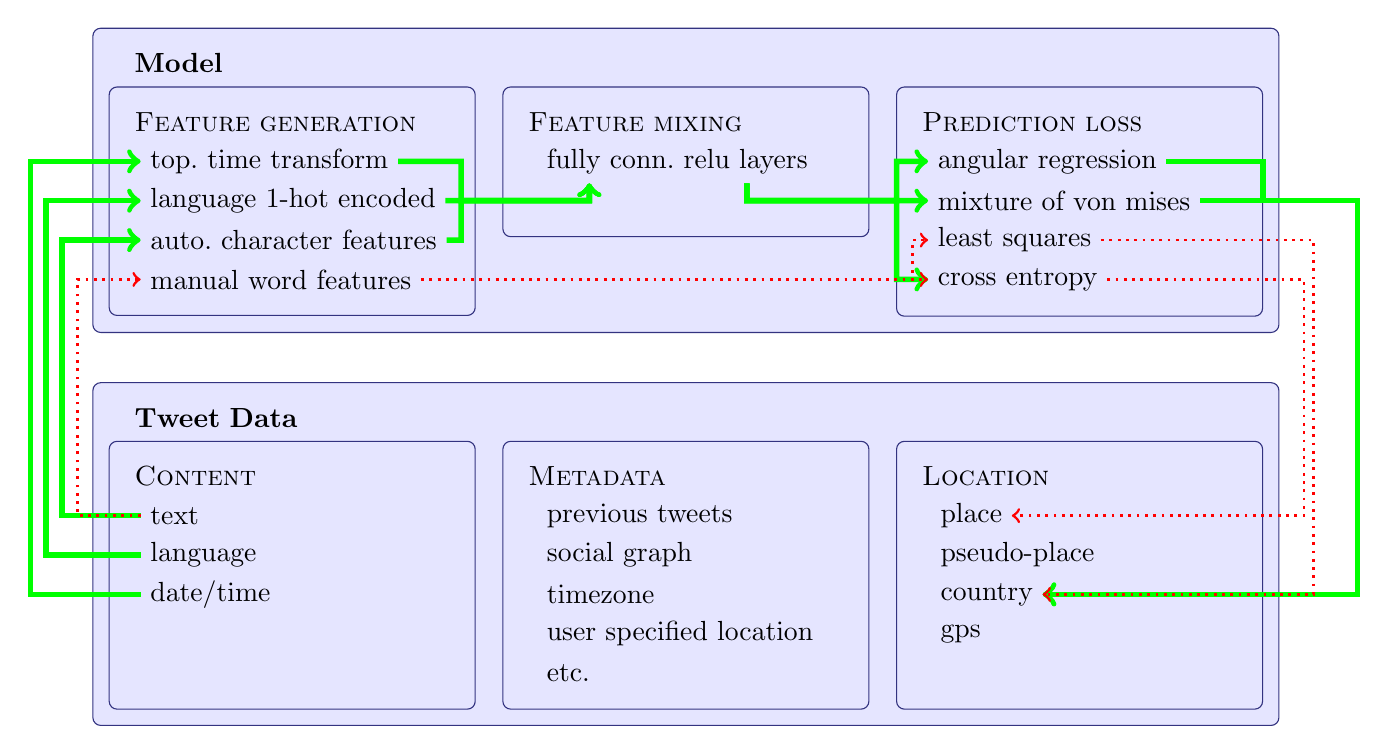
\begin{tikzpicture}
        [ node distance=5mm
        , li/.style={anchor=west}
        , l1/.style={ text width=4cm}
        , tc/.style={anchor=north, text width=4cm}
        , tc2/.style={li, minimum height=5mm}
        , box/.style={draw=border, inner sep=2mm, rounded corners=1mm}
        , us/.style  ={->,line width=2pt,draw=green}
        , them/.style={->,line width=1pt,draw=red,dotted}
        ]
        \pgfdeclarelayer{background}
        \pgfsetlayers{background,main}
        \definecolor{lightblue}{rgb}{0.9,0.9,1.0}
        \definecolor{border}{rgb}{0.2,0.2,0.5}
        \newcommand{\headerA}[1]{\textbf{#1}}
        \newcommand{\headerB}[1]{\textsc{#1}}

        \node (t) [l1]  at (0,0) {\headerA{Tweet Data}};
            \node (tc) [tc] at (0,-0.5) {\headerB{Content}};
                \node (tc0) [right=2mm of tc.west] {};
                \node (tc1) [below=of tc0.west, tc2] {text};
                \node (tc2) [below=of tc1.west, tc2] {language};
                \node (tc3) [below=of tc2.west, tc2] {date/time};
                \node (tc4) [below=of tc3.west, tc2] {};
                \node (tc5) [below=of tc4.west, tc2] {};
            \node (tcB) [box, fit={(tc)(tc5)}] {};
            \node (tm) [tc] at (5,-0.5) {\headerB{Metadata}};
                \node (tm1) [below=of tm.west , tc2] {~~previous tweets};
                \node (tm2) [below=of tm1.west, tc2] {~~social graph};
                \node (tm3) [below=of tm2.west, tc2] {~~timezone};
                \node (tm4) [below=of tm3.west, tc2] {~~user specified location};
                \node (tm5) [below=of tm4.west, tc2] {~~etc.};
            \node (tmB) [box, fit={(tm)(tm5)}] {};
            \node (tp) [tc] at (10,-0.5) {\headerB{Location}};
                \node (tp1) [below=of tp.west , tc2] {~~place};
                \node (tp2) [below=of tp1.west, tc2] {~~pseudo-place};
                \node (tp3) [below=of tp2.west, tc2] {~~country};
                \node (tp4) [below=of tp3.west, tc2] {~~gps};
                \node (tp5) [below=of tp4.west, tc2] {~~};
            \node (tpB) [box, fit={(tp)(tp5)}] {};
        \begin{pgfonlayer}{background}
            \node [box, fill=lightblue, fit={(t) (tcB) (tmB)(tpB)}] {};
        \end{pgfonlayer}

        \node (m) [l1] at (0,4.5) {\headerA{Model}};
            \node (mf) [tc] at (0,4.0) {\headerB{Feature generation}};
                \node (mf0) [right=2mm of mf.west] {};
                \node (mf1) [below=of mf0.west, tc2] {top.\ time transform};
                \node (mf2) [below=of mf1.west, tc2] {language 1-hot encoded};
                \node (mf3) [below=of mf2.west, tc2] {auto.\ character features};
                \node (mf4) [below=of mf3.west, tc2] {manual word features};
            \node (mfB) [box, fit={(mf)(mf4)}] {};
            \node (mm) [tc] at (5,4.0) {\headerB{Feature mixing}};
                \node (mm1) [below=of mm.west , tc2] {~~fully conn.\ relu layers};
                \node (mm2) [below=of mm1.west, tc2] {~~};
                %\node (mm3) [below=of mm2.west, tc2] {~~};
                %\node (mm4) [below=of mm3.west, tc2] {~~};
            \node (mmB) [box, fit={(mm)(mm2)}] {};
            \node (mp) [tc] at (10,4.0) {\headerB{Prediction loss}};
                \node (mp0) [right=2mm of mp.west] {};
                \node (mp1) [below=of mp0.west, tc2] {angular regression};
                \node (mp2) [below=of mp1.west, tc2] {mixture of von mises};
                \node (mp3) [below=of mp2.west, tc2] {least squares};
                \node (mp4) [below=of mp3.west, tc2] {cross entropy};
            \node (mpB) [box, fit={(mp)(mp4)}] {};
        \begin{pgfonlayer}{background}
            \node [box, fill=lightblue, fit={(m)(mfB)(mpB)}] {};
        \end{pgfonlayer}

        \node (tc1a) [coordinate, left=10mm of tc1.west] {};
        \draw[us] (tc1.west) -- (tc1a) |- (mf3.west);

        \node (tc2a) [coordinate, left=12mm of tc2.west] {};
        \draw[us] (tc2.west) -- (tc2a) |- (mf2.west);

        \node (tc3a) [coordinate, left=14mm of tc3.west] {};
        \draw[us] (tc3.west) -- (tc3a) |- (mf1.west);

        \node (mf2a) [coordinate, right=2mm of mf2.east] {};
        \node (mm1a) [coordinate, left=10mm of mm1.south] {};
        \node (mm1a2) [coordinate, below=2.2mm of mm1a] {};
        \draw[us] (mf1.east) -| (mf2a) -- (mm1a2) -- (mm1a);
        \draw[us] (mf2.east) -| (mf2a) -- (mm1a2) -- (mm1a);
        \draw[us] (mf3.east) -| (mf2a) -- (mm1a2) -- (mm1a);

        \node (mp2c) [coordinate, left=4mm of mp2.west] {};
        \node (mm1b) [coordinate, right=10mm of mm1.south] {};
        \node (mm1b2) [coordinate, below=2.2mm of mm1b] {};
        \draw[us] (mm1b) -- (mm1b2) -- (mp2c) |- (mp1);
        \draw[us] (mm1b) -- (mm1b2) -- (mp2c) |- (mp2);
        \draw[us] (mm1b) -- (mm1b2) -- (mp2c) |- (mp4);

        \node (mp4a) [coordinate, right=24mm of mp4.east] {};
        \node (tp1a) [coordinate, right=8mm of tp1.east] {};
        %\draw[->] (mp4) -- (mp4a) |- (tp1a) |- (tp1);
        %\draw[->] (mp4) -- (mp4a) |- (tp1a) |- (tp2);

        \node (mp2a) [coordinate, right=8mm of mp2.east] {};
        \node (mp2b) [coordinate, right=12mm of mp2a.east] {};
        \draw[us] (mp1.east) -| (mp2a) -- (mp2b) |- (tp3);
        \draw[us] (mp2.east) -| (mp2a) -- (mp2b) |- (tp3);

        \node (tc1a2) [coordinate, left=8mm of tc1.west] {};
        \draw[them] (tc1.west) -- (tc1a2) |- (mf4.west);

        \node (mp4a) [coordinate, left=2mm of mp4] {};
        \draw[them] (mf4.east) -- (mp4a) |- (mp4.west);
        \draw[them] (mf4.east) -- (mp4a) |- (mp3.west);

        \node (mp3b) [coordinate, right=27mm of mp3.east] {};
        \draw[them] (mp3.east) -- (mp3b) |- (tp3.east);
        
        \node (mp4b) [coordinate, right=25mm of mp4.east] {};
        \draw[them] (mp4.east) -- (mp4b) |- (tp1.east);

    \end{tikzpicture}
    \caption{The general model framework.}
\end{figure}

%%%%%%%%%%%%%%%%%%%%%%%%%%%%%%%%%%%%%%%%%%%%%%%%%%%%%%%%%%%%%%%%%%%%%%%%%%%%%%%
\newpage

\ignore{
\section{Problem Overview}

Previous work focuses on learning a parameterized model for tweet location.
The advantages of these methods are:
\begin{enumerate*}[label=(\arabic*)]
    \item the resulting models are simple, and
    \item the models can be trained and deployed on low-power devices.
\end{enumerate*}
The disadvantages are:
\begin{enumerate}
    \item These methods can model recurring space/time interactions 
        (e.g. patterns caused by timezone differences and weekend/nonweekend behavioral patterns), 
        but they cannot handle one time outlier events such as natural disasters or entertainment events.
    %\item They provide point estimates a tweet's location rather than a distribution of possible locations.
    \item Experiments by \citet{mahmud2014home} and \citet{dredze2016geolocation} show that the models do not generalize well to unseen time periods.
\end{enumerate}
I propose a nonparametric approach to geolocation that should improve these disadvantages.
The tradeoff is that the model is more complex and not deployable on low-power devices.

%%%%%%%%%%%%%%%%%%%%%%%%%%%%%%%%%%%%%%%%

\section{Proposed Solution}

Let $\{e_i\}_{i=1}^n$ be the set of observed tweets,
and $e$ be a new tweet not in the database.
Then define the nonparametric distribution over $e$ 
\begin{equation}
    \prob e
    \propto
    %\frac 1 n 
    \sum_{i=1}^n \exp\left(-\dist_\theta(e,e_i)^2\right)
    ,
\end{equation}
where $\dist_\theta$ is a distance metric between two tweets that depends on parameter vector $\theta$.
If we let $e(\ell)$ denote the tweet $e$ updated to have location $\ell$,
then the distribution of the tweet's location is given by
\begin{equation}
    \prob {e(\ell)} 
    \propto
    %\frac 1 n 
    \sum_{i=1}^n \exp\left(-\dist_\theta(e(\ell),e_i)^2\right)
    ,
\end{equation}
and the maximum likelihood point estimate of the tweet's location is
\begin{equation}
    \label{eq:hatell}
    \hat\ell
    =
    \argmax_{\ell} 
    \sum_{i=1}^n \exp\left(-\dist_\theta(e(\ell),e_i)^2\right)
    .
\end{equation}
The quality of the estimate $\hat\ell$ is affected by three factors:
\begin{enumerate}
    \item \emph{The number of tweets in the database.}
        Standard results in nonparametric distributions show that as $n\to\infty$, 
        the distribution $\prob{e}$ will approach the true underlying distribution.
        %Since the underlying distribution is highly complex, 
        %many samples will be needed to get a reasonable approximation.
        %Fortunately, we have many tweets available to us,
%
        The downside of this strategy is that the summations above are summations over the entire database.
        This is not practical, so the summation will need to be approximated.
        There are many good metric data structures that can restrict the summation to only the most relevant portions of the space.

    \item \emph{The family of distance metrics $\dist_\theta$.}
        The distance metric needs to tie information about a tweet's location to information about the other features in a tweet.
        There are many possible metric families,
        and finding the optimal one is likely a difficult challenge.

        A simple approach is to use an ``ensemble of metrics.''
        Let $\{d^{(i)}\}_{i=1}^m$ be a set of $m$ metrics.
        Then define the Mahalanobis distance
        \begin{equation}
            \label{eq:mahalanobis}
            \dist_\theta(e_1,e_2) ^2
            =
            \trans{
            \begin{pmatrix}
                \dist^{(1)}(e_1,e_2) \\
                \dist^{(2)}(e_1,e_2) \\
                \vdots \\
                \dist^{(m)}(e_1,e_2) \\
            \end{pmatrix}
            }
            \theta
            \begin{pmatrix}
                \dist^{(1)}(e_1,e_2) \\
                \dist^{(2)}(e_1,e_2) \\
                \vdots \\
                \dist^{(m)}(e_1,e_2) \\
            \end{pmatrix}
        \end{equation}
        %where $A : \R^{m\times m}$ is the parameter vector $\theta$ that is to be learned.
        where $\theta$ is a $m\times m$ matrix that needs to be estimated from the data.

        The ensemble should include several metrics related to gps coordinates 
        (e.g. the geodesic distance \citep{vincenty1975direct}, the google maps distance),
        time 
        (e.g. total distance in time, and the distance in time mod hourly, daily, weekly, monthly, and yearly intervals),
        social graph distances
        (e.g. total number of hops in a friendship graph),
        and any features of the tweet itself.

        There are two possible drawbacks of a large ensemble.
        First, a larger ensemble will increase the computational burden of computing distances.
        This can possibly be ameliorated by a pruning strategy that only evaluates the more expensive distances after the cheaper ones if it is actually necessary.
        Second, more metrics increases the number of parameters, increasing the possiblity of overfitting.
        The number of available tweets is so large, however, that this seems unlikely for a linear Mahalinobis distance.

        %These ensemble metrics can be extended by:

    \item \emph{The quality of the estimated parameter vector $\theta$.}
        %We can solve for $\hat\theta$ using the formula
        A good parameter vector $\hat\theta$ will maximize the likelihood that
        \begin{equation}
            \label{eq:hattheta}
            \hat\theta
            =
            \argmax_{\theta} 
            \sum_{i=1}^n 
            \sum_{j=1}^{i-1}
            \exp\left(-\dist_\theta(e_i,e_j)^2\right)
            .
        \end{equation}
        This can be solved with an SGD procedure.
        Using only a small sample of the data should be sufficient.
        %For the Mahalanobis metric above,
        %this optimization is convex.
        %In general, however, for other metrics, it need not be.
        %An important decision will be the choice of regularizer for $\theta$.
\end{enumerate}

%%%%%%%%%%%%%%%%%%%%%%%%%%%%%%%%%%%%%%%%

%\newpage
\section{Research Questions}

\noindent
Applied questions
\begin{enumerate}
    %\item \textbf{How do we efficiently perform the sums?}
    \item Does jointly training the feature space and metric parameters improve performance?
    \item Many possible choices of metric to experiment with to determine which is best for different applications.
        For example, how should we incorporate information related to ``location'' vs ``gps'' fields of the tweet?
    \item Which regularizer should be chosen to optimize $\hat\theta$ in \eqref{eq:hattheta}?
        Is there a better loss function to use?
    \item Queries in this framework can be significantly more complicated:
        \begin{enumerate}
        \item We can easily in incorporate constraints into the queries.
            For example: Given that I know the tweet came from the midwest,
            which city was it most likely to come from?
        \item Given that a tweet came from a particular location,
            what time was it most likely tweeted?
            What user mostly likely sent the tweet?
        \item
            Generate a tweet that is likely to have been sent from location X at time Y.
            (This requires that the metrics in the ensemble have a generative semantics.)
        \end{enumerate}
\end{enumerate}

\noindent
Theoretical questions:
\begin{enumerate}
    \item \emph{Nonconvex optimization.}
        The optimization in \eqref{eq:hatell} is nonconvex.
        Finding a unique global optimum, however, is not likely to be important for practitioners.
        Instead, reporting several representative solutions will likely be more useful.
        These solutions should:
        \begin{enumerate}
            \item not get stuck in ``small'' local optima, and
            \item represent all the largest modes in the distribution.
        \end{enumerate}
        What is the best way to optimize under these constraints?

    \item \emph{Metric ensembles.}
        The theoretical properties of ensembles of metrics like proposed in \eqref{eq:mahalanobis} have not been explicitly studied before.
        \begin{enumerate}
            \item How does the dimension of the ``submetrics'' influence the dimension of the resulting ensembled metric?
                It is likely that each metric will have ``different dimensions at different scales,''
                and how do we incorporate this information to improve runtime bounds on queries?
            \item What are the best ways to ensemble the metrics? 
                \begin{enumerate}
                    \item Other $L_p$ combinations can be used besides $L_2$.
                    \item The matrix $\theta$ could be replaced by a higher order tensor to capture more complicated relationships between the submetrics.
                    \item We can kernelize the Mahalanobis distance to create a nonlinear family of metrics.
                    \item Using parameterized metrics as the base metrics naturally results in a ``deep'' metric learning problem.
                \end{enumerate}
            \item Can we develop metric data structures specifically tuned for ensemble metrics?
                \begin{enumerate}
                    \item Can we efficiently add/delete/modify metrics in the ensemble without recreating the data structure?
                    \item Can we query using only a portion of the metrics in the ensemble?
                    \item Can we support database style queries distributed over multiple machines? 
                \end{enumerate}
        \end{enumerate}
\end{enumerate}

%%%%%%%%%%%%%%%%%%%%%%%%%%%%%%%%%%%%%%%%

\newpage

%%%%%%%%%%%%%%%%%%%%%%%%%%%%%%%%%%%%%%%%%%%%%%%%%%%%%%%%%%%%%%%%%%%%%%%%%%%%%%%%

\section{Problem description}

Existing work on tweet geolocation uses only text features to predict location.
I want to use time as well.

%%%%%%%%%%%%%%%%%%%%%%%%%%%%%%%%%%%%%%%%

\subsection{Intuitive motivation}

Time by itself is a good predictor of tweet location.
People are more likely to tweet during daytime hours,
and daytime is determined by longitude.
Combining time with textual features is even more powerful.

Consider a tweet with the text ``I am at the Taylor Swift concert''
(or alternatively a video of Taylor Swift performing).
If we knew the time of the tweet, 
and we knew Taylor Swift's concert schedule,
then we could get a good prediction of the location of the tweet.
Without knowing the time, however, we cannot say which city the tweet was sent from.
We actually don't even need to know Taylor Swift's concert schedule.
These concerts have many thousands of attendees, many of whom are tweeting.
If any of these attendees tweets about Taylor Swift and has geotagging enabled,
we should be able to use this information to infer that the original tweet was from the same location
(since it happened at the same time).

The example of a Taylor Swift concert happens over a narrow time scale and in a small location.
Other examples of space/time dependencies occur at larger scale.
For example: 
(i) natural disasters such as floods can affect multiple cities over many weeks;
(ii) normal weather conditions (such as snow, rain, or heat) affect latitudinal bands over the course of seasons;
and (iii) elections can affect entire cities, states, and countries for months.
We would like a system that can automatically identify these space/time dependencies and use them to predict tweet location.

%%%%%%%%%%%%%%%%%%%%%%%%%%%%%%%%%%%%%%%%

\subsection {Formal problem statement}

We call each tweet an event $e$ and decompose it into three components: 
\begin{align*}
    %g    &= \text{the gps coordinates} \\ 
    %\ell &= \text{the location (either the location field in the tweet or exact gps coordinates)} \\
    \ell : \R^2 &= \text{the location represented as gps coordinates} \\
    x    : \R^d &= \text{document features (constructed from any text/images/video/urls in the tweet)} \\
    t    : \R~ &= \text{time}
\end{align*}
%Existing approaches model the probability distribution $\cprob{\ell}{d}$.
%Existing baseline approaches estimate the distribution $\cprob{\ell}{d}$.
Our goal is to estimate the conditional distribution $\cprob{\ell}{x,t}$.

%%%%%%%%%%%%%%%%%%%%%%%%%%%%%%%%%%%%%%%%

\subsection {Proposed technique}

I propose a nonparametric model for estimating the density.
Specifically, 
\begin{equation}
    \label{eq:nonparam}
    %\prob{e} = \frac 1 n \sum_{i=1}^n k(e,e_i)
    \prob{e} = \frac 1 n \sum_{i=1}^n \exp(-\dist(e,e_i)^2)
\end{equation}
where $\dist$ is a metric distance that describes the similarity of two tweets.
Learning the model will consist of setting parameters in the distance function.
The main challenge of large scale nonparametric models is that the summation in \eqref{eq:nonparam} is over the entire data set.
A clever metric data structure will be needed so that only a small fraction of the data will need to be searched.

Many metrics can be defined between tweets,
and each metric will determine a corresponding probability distribution.
The simplest metrics for location estimation ignore all the information in the tweets except the location.
The most obvious distance function is to use the great circle distance $\dist\gcirc$ between two gps coordinates.
The obvious formula contains numerical instabilities,
and so Vincenty's formula should be used instead \citep{vincenty1975direct}.
A bandwidth parameter would need to be estimated from the data.
%More powerful distance functions would take into account the rate that information can travel between two locations.
%We can define the google maps distance $\dist\gmap$ to be the length of time that google maps says it takes to drive between two locations.
%This distance is more likely to be too expensive to compute;
%and while it may be more accurate than $\dist\gcirc$,
%it is unlikely to be the best distance measure possible.
%Ideally, we would use a metric learning algorithm to achieve the best possible metric.

I think a learned metric would be a good way to associate textual and spatial features.
If $\Dist$ is a family of metrics and $\loss$ a loss function,
then the training procedure solves
\begin{equation}
    \hat\dist = \argmin_{\dist\in\Dist} \sum_{e_1,e_2\in E} \loss(\dist(e_1,e_2))
    .
\end{equation}
As in the testing procedure, evaluating the sum is computationally expensive and clever data structures are needed to compute it efficiently.
The efficacy of the method will be determined by the choice of distance family $\Dist$.

\ignore{
If the location is independent of the document and time, then $\cprob{\ell}{x,t} = \prob{\ell}$.
This can be modeled as a mixture of $n$ isotropic Gaussians.
That is,
\begin{equation}
    \prob{\ell} = \sum_{i=1}^n w_i\normal{\mu_i}{\eye\sigma_i}
    .
\end{equation}
There are 488 cities in the worldwith at least 1 million people, 
so around 1000 seems like a reasonable choice of $n$.
The parameters $w_i$, $\mu_i$, and $\sigma_i$ must be learned from the data.

Next we incorporate a dependence on time.
Let $k : E \times E \to \R$ be a kernel function that assigns a similarity to two tweets.
As simple gaussian kernel could be
\begin{equation}
    k(e_1,e_2) 
    = \exp(-\tau\abs{e_1(t) - e_2(t)}^2
           -\lambda\ltwo{e_1(\ell) - e_2(\ell)}^2)
\end{equation}
where $\tau$ and $\lambda$ are parameters that control the influence of temporal and spatial distance in the events' similarity.
We can then define the conditional distribution
\begin{equation}
    \cprob{\ell}{t} = p(\ell)\exp(-\sum_{\substack{\text{events $e'$ s.t.}\\e'(t)<t}} k(e,e'))
    .
\end{equation}

Finally, we can incorporate a dependence on the textual features simply by updating the kernel to include a dependence on the text.
}

%A Hawkes process is an appropriate model for $\cprob{\ell}{t}$.
%In a Hawkes process,
%the likelihood of an event at location $\ell$ is high when events have recently happened in nearby locations,
%and low when events have not recently happened nearby.
%Formally,
%\begin{equation}
    %\cprob{\ell}{t} 
    %%\propto
    %=
    %\prob{\ell}\exp(-\lambda(\ell;t))
%\end{equation}
%where $\lambda$ is called the rate function and is given by
%\begin{equation}
    %\label{eq:kernel}
    %\lambda(\ell;t) = \sum_{e} k(\ell,t,e,\theta)
%\end{equation}
%where $k$ is a kernel function that depends on parameter $\theta$.

%%%%%%%%%%%%%%%%%%%%%%%%%%%%%%%%%%%%%%%%
}

\ignore{
\subsection{Computational notes}

\begin{enumerate}
    \item
        The summation in \eqref{eq:kernel} is over all tweets,
        which is obviously infeasible.
        Any reasonable choice of kernel will have a large value only for tweets nearby in space/time.
        Therefore distant points can be pruned from the summation to improve computation time.

    \item
        As formulated, the features can be computed completely independently from modeling of the space/time relations.
        It may be possible to improve the performance by jointly optimizing the feature selection algorithms with the space/time objectives.

    \item
        Modeling the locations $\ell$ as points in $\R^2$ induces distortions,
        because the data is actually gps coordinates on a sphere.
        Restricting the data to lie on the sphere would be better,
        but I'm not sure how to enforce that type of constraint.
        It might be easier (and more accurate!) to learn the topology of the underlying space from the data.
        This could help incorporate non-gps location data as well,
        and make the system usable on non-twitter data.
        For example, we could predict the university/funding agency for a piece of research in a citation social network.

    \item
        We should be able to use a semisupervised learning procedure to use all the tweets without location data.

\end{enumerate}
}

%%%%%%%%%%%%%%%%%%%%%%%%%%%%%%%%%%%%%%%%%%%%%%%%%%%%%%%%%%%%%%%%%%%%%%%%%%%%%%%%

\section{Experiments}

\begin{figure}
    % GNUPLOT: LaTeX picture with Postscript
\begingroup
  \makeatletter
  \providecommand\color[2][]{%
    \GenericError{(gnuplot) \space\space\space\@spaces}{%
      Package color not loaded in conjunction with
      terminal option `colourtext'%
    }{See the gnuplot documentation for explanation.%
    }{Either use 'blacktext' in gnuplot or load the package
      color.sty in LaTeX.}%
    \renewcommand\color[2][]{}%
  }%
  \providecommand\includegraphics[2][]{%
    \GenericError{(gnuplot) \space\space\space\@spaces}{%
      Package graphicx or graphics not loaded%
    }{See the gnuplot documentation for explanation.%
    }{The gnuplot epslatex terminal needs graphicx.sty or graphics.sty.}%
    \renewcommand\includegraphics[2][]{}%
  }%
  \providecommand\rotatebox[2]{#2}%
  \@ifundefined{ifGPcolor}{%
    \newif\ifGPcolor
    \GPcolorfalse
  }{}%
  \@ifundefined{ifGPblacktext}{%
    \newif\ifGPblacktext
    \GPblacktexttrue
  }{}%
  % define a \g@addto@macro without @ in the name:
  \let\gplgaddtomacro\g@addto@macro
  % define empty templates for all commands taking text:
  \gdef\gplbacktext{}%
  \gdef\gplfronttext{}%
  \makeatother
  \ifGPblacktext
    % no textcolor at all
    \def\colorrgb#1{}%
    \def\colorgray#1{}%
  \else
    % gray or color?
    \ifGPcolor
      \def\colorrgb#1{\color[rgb]{#1}}%
      \def\colorgray#1{\color[gray]{#1}}%
      \expandafter\def\csname LTw\endcsname{\color{white}}%
      \expandafter\def\csname LTb\endcsname{\color{black}}%
      \expandafter\def\csname LTa\endcsname{\color{black}}%
      \expandafter\def\csname LT0\endcsname{\color[rgb]{1,0,0}}%
      \expandafter\def\csname LT1\endcsname{\color[rgb]{0,1,0}}%
      \expandafter\def\csname LT2\endcsname{\color[rgb]{0,0,1}}%
      \expandafter\def\csname LT3\endcsname{\color[rgb]{1,0,1}}%
      \expandafter\def\csname LT4\endcsname{\color[rgb]{0,1,1}}%
      \expandafter\def\csname LT5\endcsname{\color[rgb]{1,1,0}}%
      \expandafter\def\csname LT6\endcsname{\color[rgb]{0,0,0}}%
      \expandafter\def\csname LT7\endcsname{\color[rgb]{1,0.3,0}}%
      \expandafter\def\csname LT8\endcsname{\color[rgb]{0.5,0.5,0.5}}%
    \else
      % gray
      \def\colorrgb#1{\color{black}}%
      \def\colorgray#1{\color[gray]{#1}}%
      \expandafter\def\csname LTw\endcsname{\color{white}}%
      \expandafter\def\csname LTb\endcsname{\color{black}}%
      \expandafter\def\csname LTa\endcsname{\color{black}}%
      \expandafter\def\csname LT0\endcsname{\color{black}}%
      \expandafter\def\csname LT1\endcsname{\color{black}}%
      \expandafter\def\csname LT2\endcsname{\color{black}}%
      \expandafter\def\csname LT3\endcsname{\color{black}}%
      \expandafter\def\csname LT4\endcsname{\color{black}}%
      \expandafter\def\csname LT5\endcsname{\color{black}}%
      \expandafter\def\csname LT6\endcsname{\color{black}}%
      \expandafter\def\csname LT7\endcsname{\color{black}}%
      \expandafter\def\csname LT8\endcsname{\color{black}}%
    \fi
  \fi
  \setlength{\unitlength}{0.0500bp}%
  \begin{picture}(5040.00,3240.00)%
    \gplgaddtomacro\gplbacktext{%
      \csname LTb\endcsname%
      \put(264,660){\makebox(0,0)[r]{\strut{}\scriptsize 0.0}}%
      \put(264,1239){\makebox(0,0)[r]{\strut{}\scriptsize 0.1}}%
      \put(264,1818){\makebox(0,0)[r]{\strut{}\scriptsize 0.2}}%
      \put(264,2396){\makebox(0,0)[r]{\strut{}\scriptsize 0.3}}%
      \put(264,2975){\makebox(0,0)[r]{\strut{}\scriptsize 0.4}}%
      \put(580,528){\rotatebox{-45}{\makebox(0,0)[l]{\strut{}\scriptsize~USA}}}%
      \put(949,528){\rotatebox{-45}{\makebox(0,0)[l]{\strut{}\scriptsize~Brazil}}}%
      \put(1318,528){\rotatebox{-45}{\makebox(0,0)[l]{\strut{}\scriptsize~Japan}}}%
      \put(1687,528){\rotatebox{-45}{\makebox(0,0)[l]{\strut{}\scriptsize~UK}}}%
      \put(2056,528){\rotatebox{-45}{\makebox(0,0)[l]{\strut{}\scriptsize~TR}}}%
      \put(2425,528){\rotatebox{-45}{\makebox(0,0)[l]{\strut{}\scriptsize~Philippines}}}%
      \put(2794,528){\rotatebox{-45}{\makebox(0,0)[l]{\strut{}\scriptsize~Argentina}}}%
      \put(3163,528){\rotatebox{-45}{\makebox(0,0)[l]{\strut{}\scriptsize~Saudi~Arabia}}}%
      \put(3532,528){\rotatebox{-45}{\makebox(0,0)[l]{\strut{}\scriptsize~Spain}}}%
      \put(3901,528){\rotatebox{-45}{\makebox(0,0)[l]{\strut{}\scriptsize~Mexico}}}%
      \put(4270,528){\rotatebox{-45}{\makebox(0,0)[l]{\strut{}\scriptsize~other}}}%
      \put(-242,1817){\rotatebox{-270}{\makebox(0,0){\strut{}\scriptsize fraction of tweets}}}%
      \put(2425,2865){\makebox(0,0){\strut{}Most Active Countries}}%
    }%
    \gplgaddtomacro\gplfronttext{%
    }%
    \gplbacktext
    \put(0,0){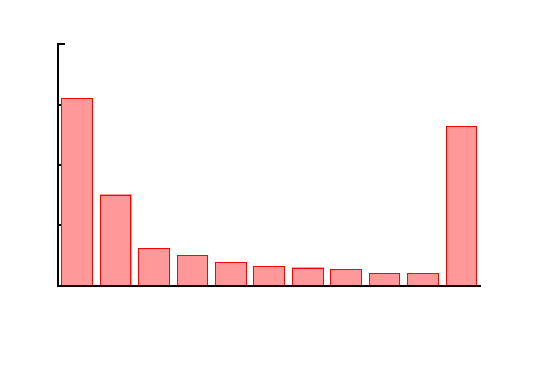
\includegraphics{img/country}}%
    \gplfronttext
  \end{picture}%
\endgroup

    % GNUPLOT: LaTeX picture with Postscript
\begingroup
  \makeatletter
  \providecommand\color[2][]{%
    \GenericError{(gnuplot) \space\space\space\@spaces}{%
      Package color not loaded in conjunction with
      terminal option `colourtext'%
    }{See the gnuplot documentation for explanation.%
    }{Either use 'blacktext' in gnuplot or load the package
      color.sty in LaTeX.}%
    \renewcommand\color[2][]{}%
  }%
  \providecommand\includegraphics[2][]{%
    \GenericError{(gnuplot) \space\space\space\@spaces}{%
      Package graphicx or graphics not loaded%
    }{See the gnuplot documentation for explanation.%
    }{The gnuplot epslatex terminal needs graphicx.sty or graphics.sty.}%
    \renewcommand\includegraphics[2][]{}%
  }%
  \providecommand\rotatebox[2]{#2}%
  \@ifundefined{ifGPcolor}{%
    \newif\ifGPcolor
    \GPcolorfalse
  }{}%
  \@ifundefined{ifGPblacktext}{%
    \newif\ifGPblacktext
    \GPblacktexttrue
  }{}%
  % define a \g@addto@macro without @ in the name:
  \let\gplgaddtomacro\g@addto@macro
  % define empty templates for all commands taking text:
  \gdef\gplbacktext{}%
  \gdef\gplfronttext{}%
  \makeatother
  \ifGPblacktext
    % no textcolor at all
    \def\colorrgb#1{}%
    \def\colorgray#1{}%
  \else
    % gray or color?
    \ifGPcolor
      \def\colorrgb#1{\color[rgb]{#1}}%
      \def\colorgray#1{\color[gray]{#1}}%
      \expandafter\def\csname LTw\endcsname{\color{white}}%
      \expandafter\def\csname LTb\endcsname{\color{black}}%
      \expandafter\def\csname LTa\endcsname{\color{black}}%
      \expandafter\def\csname LT0\endcsname{\color[rgb]{1,0,0}}%
      \expandafter\def\csname LT1\endcsname{\color[rgb]{0,1,0}}%
      \expandafter\def\csname LT2\endcsname{\color[rgb]{0,0,1}}%
      \expandafter\def\csname LT3\endcsname{\color[rgb]{1,0,1}}%
      \expandafter\def\csname LT4\endcsname{\color[rgb]{0,1,1}}%
      \expandafter\def\csname LT5\endcsname{\color[rgb]{1,1,0}}%
      \expandafter\def\csname LT6\endcsname{\color[rgb]{0,0,0}}%
      \expandafter\def\csname LT7\endcsname{\color[rgb]{1,0.3,0}}%
      \expandafter\def\csname LT8\endcsname{\color[rgb]{0.5,0.5,0.5}}%
    \else
      % gray
      \def\colorrgb#1{\color{black}}%
      \def\colorgray#1{\color[gray]{#1}}%
      \expandafter\def\csname LTw\endcsname{\color{white}}%
      \expandafter\def\csname LTb\endcsname{\color{black}}%
      \expandafter\def\csname LTa\endcsname{\color{black}}%
      \expandafter\def\csname LT0\endcsname{\color{black}}%
      \expandafter\def\csname LT1\endcsname{\color{black}}%
      \expandafter\def\csname LT2\endcsname{\color{black}}%
      \expandafter\def\csname LT3\endcsname{\color{black}}%
      \expandafter\def\csname LT4\endcsname{\color{black}}%
      \expandafter\def\csname LT5\endcsname{\color{black}}%
      \expandafter\def\csname LT6\endcsname{\color{black}}%
      \expandafter\def\csname LT7\endcsname{\color{black}}%
      \expandafter\def\csname LT8\endcsname{\color{black}}%
    \fi
  \fi
  \setlength{\unitlength}{0.0500bp}%
  \begin{picture}(5040.00,3240.00)%
    \gplgaddtomacro\gplbacktext{%
      \csname LTb\endcsname%
      \put(264,660){\makebox(0,0)[r]{\strut{}\scriptsize 0.0}}%
      \put(264,1123){\makebox(0,0)[r]{\strut{}\scriptsize 0.1}}%
      \put(264,1586){\makebox(0,0)[r]{\strut{}\scriptsize 0.2}}%
      \put(264,2049){\makebox(0,0)[r]{\strut{}\scriptsize 0.3}}%
      \put(264,2512){\makebox(0,0)[r]{\strut{}\scriptsize 0.4}}%
      \put(264,2975){\makebox(0,0)[r]{\strut{}\scriptsize 0.5}}%
      \put(580,528){\rotatebox{-45}{\makebox(0,0)[l]{\strut{}\scriptsize~English}}}%
      \put(949,528){\rotatebox{-45}{\makebox(0,0)[l]{\strut{}\scriptsize~Portuguese}}}%
      \put(1318,528){\rotatebox{-45}{\makebox(0,0)[l]{\strut{}\scriptsize~Spanish}}}%
      \put(1687,528){\rotatebox{-45}{\makebox(0,0)[l]{\strut{}\scriptsize~Unknown$^*$}}}%
      \put(2056,528){\rotatebox{-45}{\makebox(0,0)[l]{\strut{}\scriptsize~Japanese}}}%
      \put(2425,528){\rotatebox{-45}{\makebox(0,0)[l]{\strut{}\scriptsize~Arabic}}}%
      \put(2794,528){\rotatebox{-45}{\makebox(0,0)[l]{\strut{}\scriptsize~Turkish}}}%
      \put(3163,528){\rotatebox{-45}{\makebox(0,0)[l]{\strut{}\scriptsize~Indonesian}}}%
      \put(3532,528){\rotatebox{-45}{\makebox(0,0)[l]{\strut{}\scriptsize~Tagalog}}}%
      \put(3901,528){\rotatebox{-45}{\makebox(0,0)[l]{\strut{}\scriptsize~French}}}%
      \put(4270,528){\rotatebox{-45}{\makebox(0,0)[l]{\strut{}\scriptsize~other}}}%
      \put(-242,1817){\rotatebox{-270}{\makebox(0,0){\strut{}\scriptsize fraction of tweets}}}%
      \put(2425,2865){\makebox(0,0){\strut{}Most Active Languages}}%
    }%
    \gplgaddtomacro\gplfronttext{%
    }%
    \gplbacktext
    \put(0,0){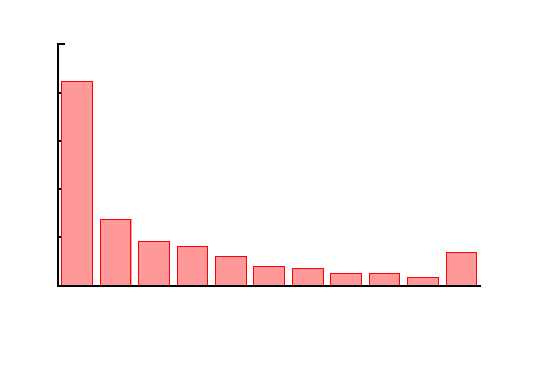
\includegraphics{img/lang}}%
    \gplfronttext
  \end{picture}%
\endgroup

    \caption{blurp}
\end{figure}

\newpage
\appendix
\section{Languages and Time of Day}
\noindent% GNUPLOT: LaTeX picture with Postscript
\begingroup
  \makeatletter
  \providecommand\color[2][]{%
    \GenericError{(gnuplot) \space\space\space\@spaces}{%
      Package color not loaded in conjunction with
      terminal option `colourtext'%
    }{See the gnuplot documentation for explanation.%
    }{Either use 'blacktext' in gnuplot or load the package
      color.sty in LaTeX.}%
    \renewcommand\color[2][]{}%
  }%
  \providecommand\includegraphics[2][]{%
    \GenericError{(gnuplot) \space\space\space\@spaces}{%
      Package graphicx or graphics not loaded%
    }{See the gnuplot documentation for explanation.%
    }{The gnuplot epslatex terminal needs graphicx.sty or graphics.sty.}%
    \renewcommand\includegraphics[2][]{}%
  }%
  \providecommand\rotatebox[2]{#2}%
  \@ifundefined{ifGPcolor}{%
    \newif\ifGPcolor
    \GPcolorfalse
  }{}%
  \@ifundefined{ifGPblacktext}{%
    \newif\ifGPblacktext
    \GPblacktexttrue
  }{}%
  % define a \g@addto@macro without @ in the name:
  \let\gplgaddtomacro\g@addto@macro
  % define empty templates for all commands taking text:
  \gdef\gplbacktext{}%
  \gdef\gplfronttext{}%
  \makeatother
  \ifGPblacktext
    % no textcolor at all
    \def\colorrgb#1{}%
    \def\colorgray#1{}%
  \else
    % gray or color?
    \ifGPcolor
      \def\colorrgb#1{\color[rgb]{#1}}%
      \def\colorgray#1{\color[gray]{#1}}%
      \expandafter\def\csname LTw\endcsname{\color{white}}%
      \expandafter\def\csname LTb\endcsname{\color{black}}%
      \expandafter\def\csname LTa\endcsname{\color{black}}%
      \expandafter\def\csname LT0\endcsname{\color[rgb]{1,0,0}}%
      \expandafter\def\csname LT1\endcsname{\color[rgb]{0,1,0}}%
      \expandafter\def\csname LT2\endcsname{\color[rgb]{0,0,1}}%
      \expandafter\def\csname LT3\endcsname{\color[rgb]{1,0,1}}%
      \expandafter\def\csname LT4\endcsname{\color[rgb]{0,1,1}}%
      \expandafter\def\csname LT5\endcsname{\color[rgb]{1,1,0}}%
      \expandafter\def\csname LT6\endcsname{\color[rgb]{0,0,0}}%
      \expandafter\def\csname LT7\endcsname{\color[rgb]{1,0.3,0}}%
      \expandafter\def\csname LT8\endcsname{\color[rgb]{0.5,0.5,0.5}}%
    \else
      % gray
      \def\colorrgb#1{\color{black}}%
      \def\colorgray#1{\color[gray]{#1}}%
      \expandafter\def\csname LTw\endcsname{\color{white}}%
      \expandafter\def\csname LTb\endcsname{\color{black}}%
      \expandafter\def\csname LTa\endcsname{\color{black}}%
      \expandafter\def\csname LT0\endcsname{\color{black}}%
      \expandafter\def\csname LT1\endcsname{\color{black}}%
      \expandafter\def\csname LT2\endcsname{\color{black}}%
      \expandafter\def\csname LT3\endcsname{\color{black}}%
      \expandafter\def\csname LT4\endcsname{\color{black}}%
      \expandafter\def\csname LT5\endcsname{\color{black}}%
      \expandafter\def\csname LT6\endcsname{\color{black}}%
      \expandafter\def\csname LT7\endcsname{\color{black}}%
      \expandafter\def\csname LT8\endcsname{\color{black}}%
    \fi
  \fi
  \setlength{\unitlength}{0.0500bp}%
  \begin{picture}(10080.00,2520.00)%
    \gplgaddtomacro\gplbacktext{%
      \csname LTb\endcsname%
      \put(176,1281){\rotatebox{-270}{\makebox(0,0){\strut{}\scriptsize fraction of tweets}}}%
      \put(3779,154){\makebox(0,0){\strut{}\scriptsize time of day (UTC)}}%
      \put(3779,2189){\makebox(0,0){\strut{}Countries that Tweet in Arabic}}%
    }%
    \gplgaddtomacro\gplfronttext{%
      \csname LTb\endcsname%
      \put(396,374){\makebox(0,0){\strut{}\scriptsize 0:00}}%
      \put(1242,374){\makebox(0,0){\strut{}\scriptsize 3:00}}%
      \put(2088,374){\makebox(0,0){\strut{}\scriptsize 6:00}}%
      \put(2934,374){\makebox(0,0){\strut{}\scriptsize 9:00}}%
      \put(3780,374){\makebox(0,0){\strut{}\scriptsize 12:00}}%
      \put(4625,374){\makebox(0,0){\strut{}\scriptsize 15:00}}%
      \put(5471,374){\makebox(0,0){\strut{}\scriptsize 18:00}}%
      \put(6317,374){\makebox(0,0){\strut{}\scriptsize 21:00}}%
      \put(7163,374){\makebox(0,0){\strut{}\scriptsize 24:00}}%
    }%
    \gplgaddtomacro\gplbacktext{%
      \csname LTb\endcsname%
      \put(9083,154){\makebox(0,0){\strut{}~~}}%
      \put(9083,2189){\makebox(0,0){\strut{} }}%
    }%
    \gplgaddtomacro\gplfronttext{%
      \csname LTb\endcsname%
      \put(8352,751){\makebox(0,0)[r]{\strut{}\scriptsize~Saudi~Arabia}}%
      \put(8352,868){\makebox(0,0)[r]{\strut{}\scriptsize~Kuwait}}%
      \put(8352,985){\makebox(0,0)[r]{\strut{}\scriptsize~Egypt}}%
      \put(8352,1102){\makebox(0,0)[r]{\strut{}\scriptsize~Arab~Emirates}}%
      \put(8352,1219){\makebox(0,0)[r]{\strut{}\scriptsize~Oman}}%
      \put(8352,1337){\makebox(0,0)[r]{\strut{}\scriptsize~Qatar}}%
      \put(8352,1454){\makebox(0,0)[r]{\strut{}\scriptsize~Bahrain}}%
      \put(8352,1571){\makebox(0,0)[r]{\strut{}\scriptsize~USA}}%
      \put(8352,1688){\makebox(0,0)[r]{\strut{}\scriptsize~UK}}%
      \put(8352,1805){\makebox(0,0)[r]{\strut{}\scriptsize~LY}}%
      \put(8352,1922){\makebox(0,0)[r]{\strut{}\scriptsize~other}}%
    }%
    \gplbacktext
    \put(0,0){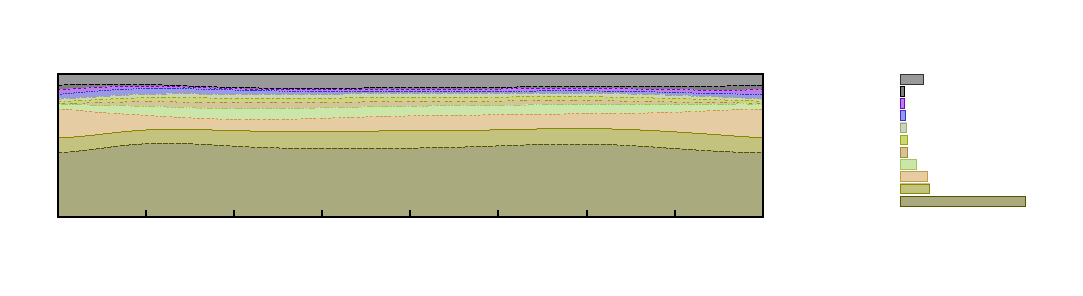
\includegraphics{img/ar}}%
    \gplfronttext
  \end{picture}%
\endgroup


\noindent% GNUPLOT: LaTeX picture with Postscript
\begingroup
  \makeatletter
  \providecommand\color[2][]{%
    \GenericError{(gnuplot) \space\space\space\@spaces}{%
      Package color not loaded in conjunction with
      terminal option `colourtext'%
    }{See the gnuplot documentation for explanation.%
    }{Either use 'blacktext' in gnuplot or load the package
      color.sty in LaTeX.}%
    \renewcommand\color[2][]{}%
  }%
  \providecommand\includegraphics[2][]{%
    \GenericError{(gnuplot) \space\space\space\@spaces}{%
      Package graphicx or graphics not loaded%
    }{See the gnuplot documentation for explanation.%
    }{The gnuplot epslatex terminal needs graphicx.sty or graphics.sty.}%
    \renewcommand\includegraphics[2][]{}%
  }%
  \providecommand\rotatebox[2]{#2}%
  \@ifundefined{ifGPcolor}{%
    \newif\ifGPcolor
    \GPcolorfalse
  }{}%
  \@ifundefined{ifGPblacktext}{%
    \newif\ifGPblacktext
    \GPblacktexttrue
  }{}%
  % define a \g@addto@macro without @ in the name:
  \let\gplgaddtomacro\g@addto@macro
  % define empty templates for all commands taking text:
  \gdef\gplbacktext{}%
  \gdef\gplfronttext{}%
  \makeatother
  \ifGPblacktext
    % no textcolor at all
    \def\colorrgb#1{}%
    \def\colorgray#1{}%
  \else
    % gray or color?
    \ifGPcolor
      \def\colorrgb#1{\color[rgb]{#1}}%
      \def\colorgray#1{\color[gray]{#1}}%
      \expandafter\def\csname LTw\endcsname{\color{white}}%
      \expandafter\def\csname LTb\endcsname{\color{black}}%
      \expandafter\def\csname LTa\endcsname{\color{black}}%
      \expandafter\def\csname LT0\endcsname{\color[rgb]{1,0,0}}%
      \expandafter\def\csname LT1\endcsname{\color[rgb]{0,1,0}}%
      \expandafter\def\csname LT2\endcsname{\color[rgb]{0,0,1}}%
      \expandafter\def\csname LT3\endcsname{\color[rgb]{1,0,1}}%
      \expandafter\def\csname LT4\endcsname{\color[rgb]{0,1,1}}%
      \expandafter\def\csname LT5\endcsname{\color[rgb]{1,1,0}}%
      \expandafter\def\csname LT6\endcsname{\color[rgb]{0,0,0}}%
      \expandafter\def\csname LT7\endcsname{\color[rgb]{1,0.3,0}}%
      \expandafter\def\csname LT8\endcsname{\color[rgb]{0.5,0.5,0.5}}%
    \else
      % gray
      \def\colorrgb#1{\color{black}}%
      \def\colorgray#1{\color[gray]{#1}}%
      \expandafter\def\csname LTw\endcsname{\color{white}}%
      \expandafter\def\csname LTb\endcsname{\color{black}}%
      \expandafter\def\csname LTa\endcsname{\color{black}}%
      \expandafter\def\csname LT0\endcsname{\color{black}}%
      \expandafter\def\csname LT1\endcsname{\color{black}}%
      \expandafter\def\csname LT2\endcsname{\color{black}}%
      \expandafter\def\csname LT3\endcsname{\color{black}}%
      \expandafter\def\csname LT4\endcsname{\color{black}}%
      \expandafter\def\csname LT5\endcsname{\color{black}}%
      \expandafter\def\csname LT6\endcsname{\color{black}}%
      \expandafter\def\csname LT7\endcsname{\color{black}}%
      \expandafter\def\csname LT8\endcsname{\color{black}}%
    \fi
  \fi
  \setlength{\unitlength}{0.0500bp}%
  \begin{picture}(10080.00,2520.00)%
    \gplgaddtomacro\gplbacktext{%
      \csname LTb\endcsname%
      \put(176,1281){\rotatebox{-270}{\makebox(0,0){\strut{}\scriptsize fraction of tweets}}}%
      \put(3779,154){\makebox(0,0){\strut{}\scriptsize time of day (UTC)}}%
      \put(3779,2189){\makebox(0,0){\strut{}Countries that Tweet in English}}%
    }%
    \gplgaddtomacro\gplfronttext{%
      \csname LTb\endcsname%
      \put(396,374){\makebox(0,0){\strut{}\scriptsize 0:00}}%
      \put(1242,374){\makebox(0,0){\strut{}\scriptsize 3:00}}%
      \put(2088,374){\makebox(0,0){\strut{}\scriptsize 6:00}}%
      \put(2934,374){\makebox(0,0){\strut{}\scriptsize 9:00}}%
      \put(3780,374){\makebox(0,0){\strut{}\scriptsize 12:00}}%
      \put(4625,374){\makebox(0,0){\strut{}\scriptsize 15:00}}%
      \put(5471,374){\makebox(0,0){\strut{}\scriptsize 18:00}}%
      \put(6317,374){\makebox(0,0){\strut{}\scriptsize 21:00}}%
      \put(7163,374){\makebox(0,0){\strut{}\scriptsize 24:00}}%
    }%
    \gplgaddtomacro\gplbacktext{%
      \csname LTb\endcsname%
      \put(9083,154){\makebox(0,0){\strut{}~~}}%
      \put(9083,2189){\makebox(0,0){\strut{} }}%
    }%
    \gplgaddtomacro\gplfronttext{%
      \csname LTb\endcsname%
      \put(8352,751){\makebox(0,0)[r]{\strut{}\scriptsize~USA}}%
      \put(8352,868){\makebox(0,0)[r]{\strut{}\scriptsize~UK}}%
      \put(8352,985){\makebox(0,0)[r]{\strut{}\scriptsize~Canada}}%
      \put(8352,1102){\makebox(0,0)[r]{\strut{}\scriptsize~Philippines}}%
      \put(8352,1219){\makebox(0,0)[r]{\strut{}\scriptsize~South~Africa}}%
      \put(8352,1337){\makebox(0,0)[r]{\strut{}\scriptsize~India}}%
      \put(8352,1454){\makebox(0,0)[r]{\strut{}\scriptsize~Australia}}%
      \put(8352,1571){\makebox(0,0)[r]{\strut{}\scriptsize~Nigeria}}%
      \put(8352,1688){\makebox(0,0)[r]{\strut{}\scriptsize~Malasia}}%
      \put(8352,1805){\makebox(0,0)[r]{\strut{}\scriptsize~Ireland}}%
      \put(8352,1922){\makebox(0,0)[r]{\strut{}\scriptsize~other}}%
    }%
    \gplbacktext
    \put(0,0){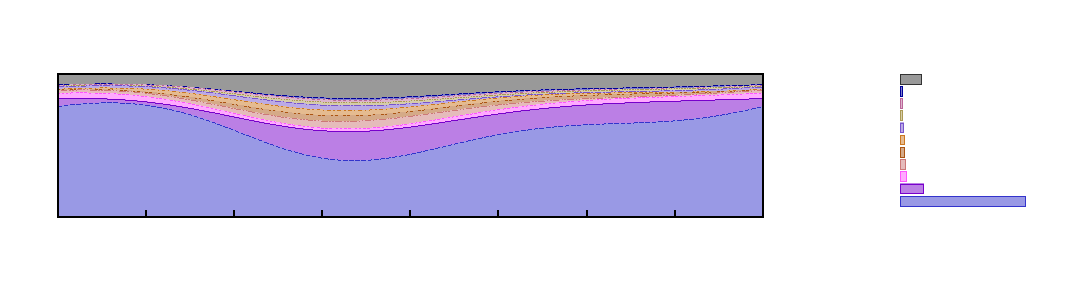
\includegraphics{img/en}}%
    \gplfronttext
  \end{picture}%
\endgroup


\noindent% GNUPLOT: LaTeX picture with Postscript
\begingroup
  \makeatletter
  \providecommand\color[2][]{%
    \GenericError{(gnuplot) \space\space\space\@spaces}{%
      Package color not loaded in conjunction with
      terminal option `colourtext'%
    }{See the gnuplot documentation for explanation.%
    }{Either use 'blacktext' in gnuplot or load the package
      color.sty in LaTeX.}%
    \renewcommand\color[2][]{}%
  }%
  \providecommand\includegraphics[2][]{%
    \GenericError{(gnuplot) \space\space\space\@spaces}{%
      Package graphicx or graphics not loaded%
    }{See the gnuplot documentation for explanation.%
    }{The gnuplot epslatex terminal needs graphicx.sty or graphics.sty.}%
    \renewcommand\includegraphics[2][]{}%
  }%
  \providecommand\rotatebox[2]{#2}%
  \@ifundefined{ifGPcolor}{%
    \newif\ifGPcolor
    \GPcolorfalse
  }{}%
  \@ifundefined{ifGPblacktext}{%
    \newif\ifGPblacktext
    \GPblacktexttrue
  }{}%
  % define a \g@addto@macro without @ in the name:
  \let\gplgaddtomacro\g@addto@macro
  % define empty templates for all commands taking text:
  \gdef\gplbacktext{}%
  \gdef\gplfronttext{}%
  \makeatother
  \ifGPblacktext
    % no textcolor at all
    \def\colorrgb#1{}%
    \def\colorgray#1{}%
  \else
    % gray or color?
    \ifGPcolor
      \def\colorrgb#1{\color[rgb]{#1}}%
      \def\colorgray#1{\color[gray]{#1}}%
      \expandafter\def\csname LTw\endcsname{\color{white}}%
      \expandafter\def\csname LTb\endcsname{\color{black}}%
      \expandafter\def\csname LTa\endcsname{\color{black}}%
      \expandafter\def\csname LT0\endcsname{\color[rgb]{1,0,0}}%
      \expandafter\def\csname LT1\endcsname{\color[rgb]{0,1,0}}%
      \expandafter\def\csname LT2\endcsname{\color[rgb]{0,0,1}}%
      \expandafter\def\csname LT3\endcsname{\color[rgb]{1,0,1}}%
      \expandafter\def\csname LT4\endcsname{\color[rgb]{0,1,1}}%
      \expandafter\def\csname LT5\endcsname{\color[rgb]{1,1,0}}%
      \expandafter\def\csname LT6\endcsname{\color[rgb]{0,0,0}}%
      \expandafter\def\csname LT7\endcsname{\color[rgb]{1,0.3,0}}%
      \expandafter\def\csname LT8\endcsname{\color[rgb]{0.5,0.5,0.5}}%
    \else
      % gray
      \def\colorrgb#1{\color{black}}%
      \def\colorgray#1{\color[gray]{#1}}%
      \expandafter\def\csname LTw\endcsname{\color{white}}%
      \expandafter\def\csname LTb\endcsname{\color{black}}%
      \expandafter\def\csname LTa\endcsname{\color{black}}%
      \expandafter\def\csname LT0\endcsname{\color{black}}%
      \expandafter\def\csname LT1\endcsname{\color{black}}%
      \expandafter\def\csname LT2\endcsname{\color{black}}%
      \expandafter\def\csname LT3\endcsname{\color{black}}%
      \expandafter\def\csname LT4\endcsname{\color{black}}%
      \expandafter\def\csname LT5\endcsname{\color{black}}%
      \expandafter\def\csname LT6\endcsname{\color{black}}%
      \expandafter\def\csname LT7\endcsname{\color{black}}%
      \expandafter\def\csname LT8\endcsname{\color{black}}%
    \fi
  \fi
  \setlength{\unitlength}{0.0500bp}%
  \begin{picture}(10080.00,2520.00)%
    \gplgaddtomacro\gplbacktext{%
      \csname LTb\endcsname%
      \put(176,1281){\rotatebox{-270}{\makebox(0,0){\strut{}\scriptsize fraction of tweets}}}%
      \put(3779,154){\makebox(0,0){\strut{}\scriptsize time of day (UTC)}}%
      \put(3779,2189){\makebox(0,0){\strut{}Countries that Tweet in Spanish}}%
    }%
    \gplgaddtomacro\gplfronttext{%
      \csname LTb\endcsname%
      \put(396,374){\makebox(0,0){\strut{}\scriptsize 0:00}}%
      \put(1242,374){\makebox(0,0){\strut{}\scriptsize 3:00}}%
      \put(2088,374){\makebox(0,0){\strut{}\scriptsize 6:00}}%
      \put(2934,374){\makebox(0,0){\strut{}\scriptsize 9:00}}%
      \put(3780,374){\makebox(0,0){\strut{}\scriptsize 12:00}}%
      \put(4625,374){\makebox(0,0){\strut{}\scriptsize 15:00}}%
      \put(5471,374){\makebox(0,0){\strut{}\scriptsize 18:00}}%
      \put(6317,374){\makebox(0,0){\strut{}\scriptsize 21:00}}%
      \put(7163,374){\makebox(0,0){\strut{}\scriptsize 24:00}}%
    }%
    \gplgaddtomacro\gplbacktext{%
      \csname LTb\endcsname%
      \put(9083,154){\makebox(0,0){\strut{}~~}}%
      \put(9083,2189){\makebox(0,0){\strut{} }}%
    }%
    \gplgaddtomacro\gplfronttext{%
      \csname LTb\endcsname%
      \put(8352,751){\makebox(0,0)[r]{\strut{}\scriptsize~Argentina}}%
      \put(8352,868){\makebox(0,0)[r]{\strut{}\scriptsize~Mexico}}%
      \put(8352,985){\makebox(0,0)[r]{\strut{}\scriptsize~Spain}}%
      \put(8352,1102){\makebox(0,0)[r]{\strut{}\scriptsize~Colombia}}%
      \put(8352,1219){\makebox(0,0)[r]{\strut{}\scriptsize~Chile}}%
      \put(8352,1337){\makebox(0,0)[r]{\strut{}\scriptsize~USA}}%
      \put(8352,1454){\makebox(0,0)[r]{\strut{}\scriptsize~Brazil}}%
      \put(8352,1571){\makebox(0,0)[r]{\strut{}\scriptsize~Uruguay}}%
      \put(8352,1688){\makebox(0,0)[r]{\strut{}\scriptsize~Venezuela}}%
      \put(8352,1805){\makebox(0,0)[r]{\strut{}\scriptsize~Ecuador}}%
      \put(8352,1922){\makebox(0,0)[r]{\strut{}\scriptsize~other}}%
    }%
    \gplbacktext
    \put(0,0){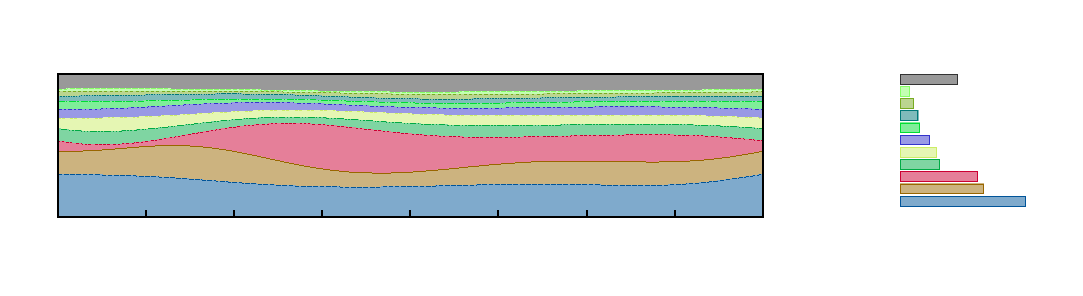
\includegraphics{img/es}}%
    \gplfronttext
  \end{picture}%
\endgroup


\noindent% GNUPLOT: LaTeX picture with Postscript
\begingroup
  \makeatletter
  \providecommand\color[2][]{%
    \GenericError{(gnuplot) \space\space\space\@spaces}{%
      Package color not loaded in conjunction with
      terminal option `colourtext'%
    }{See the gnuplot documentation for explanation.%
    }{Either use 'blacktext' in gnuplot or load the package
      color.sty in LaTeX.}%
    \renewcommand\color[2][]{}%
  }%
  \providecommand\includegraphics[2][]{%
    \GenericError{(gnuplot) \space\space\space\@spaces}{%
      Package graphicx or graphics not loaded%
    }{See the gnuplot documentation for explanation.%
    }{The gnuplot epslatex terminal needs graphicx.sty or graphics.sty.}%
    \renewcommand\includegraphics[2][]{}%
  }%
  \providecommand\rotatebox[2]{#2}%
  \@ifundefined{ifGPcolor}{%
    \newif\ifGPcolor
    \GPcolorfalse
  }{}%
  \@ifundefined{ifGPblacktext}{%
    \newif\ifGPblacktext
    \GPblacktexttrue
  }{}%
  % define a \g@addto@macro without @ in the name:
  \let\gplgaddtomacro\g@addto@macro
  % define empty templates for all commands taking text:
  \gdef\gplbacktext{}%
  \gdef\gplfronttext{}%
  \makeatother
  \ifGPblacktext
    % no textcolor at all
    \def\colorrgb#1{}%
    \def\colorgray#1{}%
  \else
    % gray or color?
    \ifGPcolor
      \def\colorrgb#1{\color[rgb]{#1}}%
      \def\colorgray#1{\color[gray]{#1}}%
      \expandafter\def\csname LTw\endcsname{\color{white}}%
      \expandafter\def\csname LTb\endcsname{\color{black}}%
      \expandafter\def\csname LTa\endcsname{\color{black}}%
      \expandafter\def\csname LT0\endcsname{\color[rgb]{1,0,0}}%
      \expandafter\def\csname LT1\endcsname{\color[rgb]{0,1,0}}%
      \expandafter\def\csname LT2\endcsname{\color[rgb]{0,0,1}}%
      \expandafter\def\csname LT3\endcsname{\color[rgb]{1,0,1}}%
      \expandafter\def\csname LT4\endcsname{\color[rgb]{0,1,1}}%
      \expandafter\def\csname LT5\endcsname{\color[rgb]{1,1,0}}%
      \expandafter\def\csname LT6\endcsname{\color[rgb]{0,0,0}}%
      \expandafter\def\csname LT7\endcsname{\color[rgb]{1,0.3,0}}%
      \expandafter\def\csname LT8\endcsname{\color[rgb]{0.5,0.5,0.5}}%
    \else
      % gray
      \def\colorrgb#1{\color{black}}%
      \def\colorgray#1{\color[gray]{#1}}%
      \expandafter\def\csname LTw\endcsname{\color{white}}%
      \expandafter\def\csname LTb\endcsname{\color{black}}%
      \expandafter\def\csname LTa\endcsname{\color{black}}%
      \expandafter\def\csname LT0\endcsname{\color{black}}%
      \expandafter\def\csname LT1\endcsname{\color{black}}%
      \expandafter\def\csname LT2\endcsname{\color{black}}%
      \expandafter\def\csname LT3\endcsname{\color{black}}%
      \expandafter\def\csname LT4\endcsname{\color{black}}%
      \expandafter\def\csname LT5\endcsname{\color{black}}%
      \expandafter\def\csname LT6\endcsname{\color{black}}%
      \expandafter\def\csname LT7\endcsname{\color{black}}%
      \expandafter\def\csname LT8\endcsname{\color{black}}%
    \fi
  \fi
  \setlength{\unitlength}{0.0500bp}%
  \begin{picture}(10080.00,2520.00)%
    \gplgaddtomacro\gplbacktext{%
      \csname LTb\endcsname%
      \put(176,1281){\rotatebox{-270}{\makebox(0,0){\strut{}\scriptsize fraction of tweets}}}%
      \put(3779,154){\makebox(0,0){\strut{}\scriptsize time of day (UTC)}}%
      \put(3779,2189){\makebox(0,0){\strut{}Countries that Tweet in French}}%
    }%
    \gplgaddtomacro\gplfronttext{%
      \csname LTb\endcsname%
      \put(396,374){\makebox(0,0){\strut{}\scriptsize 0:00}}%
      \put(1242,374){\makebox(0,0){\strut{}\scriptsize 3:00}}%
      \put(2088,374){\makebox(0,0){\strut{}\scriptsize 6:00}}%
      \put(2934,374){\makebox(0,0){\strut{}\scriptsize 9:00}}%
      \put(3780,374){\makebox(0,0){\strut{}\scriptsize 12:00}}%
      \put(4625,374){\makebox(0,0){\strut{}\scriptsize 15:00}}%
      \put(5471,374){\makebox(0,0){\strut{}\scriptsize 18:00}}%
      \put(6317,374){\makebox(0,0){\strut{}\scriptsize 21:00}}%
      \put(7163,374){\makebox(0,0){\strut{}\scriptsize 24:00}}%
    }%
    \gplgaddtomacro\gplbacktext{%
      \csname LTb\endcsname%
      \put(9083,154){\makebox(0,0){\strut{}~~}}%
      \put(9083,2189){\makebox(0,0){\strut{} }}%
    }%
    \gplgaddtomacro\gplfronttext{%
      \csname LTb\endcsname%
      \put(8352,751){\makebox(0,0)[r]{\strut{}\scriptsize~France}}%
      \put(8352,868){\makebox(0,0)[r]{\strut{}\scriptsize~USA}}%
      \put(8352,985){\makebox(0,0)[r]{\strut{}\scriptsize~Canada}}%
      \put(8352,1102){\makebox(0,0)[r]{\strut{}\scriptsize~Belgium}}%
      \put(8352,1219){\makebox(0,0)[r]{\strut{}\scriptsize~Brazil}}%
      \put(8352,1337){\makebox(0,0)[r]{\strut{}\scriptsize~UK}}%
      \put(8352,1454){\makebox(0,0)[r]{\strut{}\scriptsize~Spain}}%
      \put(8352,1571){\makebox(0,0)[r]{\strut{}\scriptsize~Cameroon}}%
      \put(8352,1688){\makebox(0,0)[r]{\strut{}\scriptsize~Switzerland}}%
      \put(8352,1805){\makebox(0,0)[r]{\strut{}\scriptsize~Cote~d'Ivoire}}%
      \put(8352,1922){\makebox(0,0)[r]{\strut{}\scriptsize~other}}%
    }%
    \gplbacktext
    \put(0,0){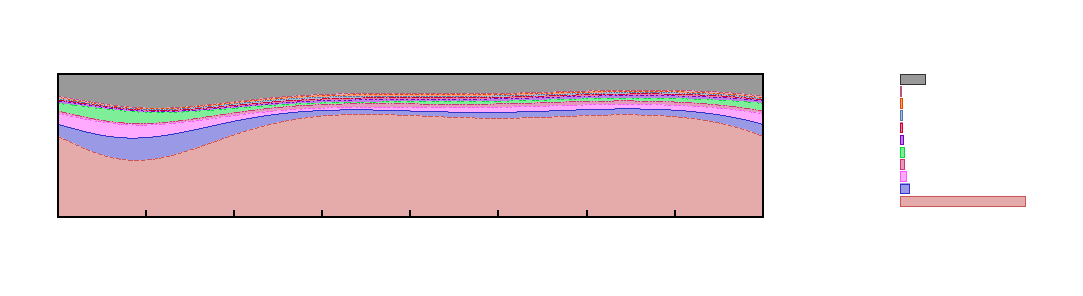
\includegraphics{img/fr}}%
    \gplfronttext
  \end{picture}%
\endgroup


\noindent% GNUPLOT: LaTeX picture with Postscript
\begingroup
  \makeatletter
  \providecommand\color[2][]{%
    \GenericError{(gnuplot) \space\space\space\@spaces}{%
      Package color not loaded in conjunction with
      terminal option `colourtext'%
    }{See the gnuplot documentation for explanation.%
    }{Either use 'blacktext' in gnuplot or load the package
      color.sty in LaTeX.}%
    \renewcommand\color[2][]{}%
  }%
  \providecommand\includegraphics[2][]{%
    \GenericError{(gnuplot) \space\space\space\@spaces}{%
      Package graphicx or graphics not loaded%
    }{See the gnuplot documentation for explanation.%
    }{The gnuplot epslatex terminal needs graphicx.sty or graphics.sty.}%
    \renewcommand\includegraphics[2][]{}%
  }%
  \providecommand\rotatebox[2]{#2}%
  \@ifundefined{ifGPcolor}{%
    \newif\ifGPcolor
    \GPcolorfalse
  }{}%
  \@ifundefined{ifGPblacktext}{%
    \newif\ifGPblacktext
    \GPblacktexttrue
  }{}%
  % define a \g@addto@macro without @ in the name:
  \let\gplgaddtomacro\g@addto@macro
  % define empty templates for all commands taking text:
  \gdef\gplbacktext{}%
  \gdef\gplfronttext{}%
  \makeatother
  \ifGPblacktext
    % no textcolor at all
    \def\colorrgb#1{}%
    \def\colorgray#1{}%
  \else
    % gray or color?
    \ifGPcolor
      \def\colorrgb#1{\color[rgb]{#1}}%
      \def\colorgray#1{\color[gray]{#1}}%
      \expandafter\def\csname LTw\endcsname{\color{white}}%
      \expandafter\def\csname LTb\endcsname{\color{black}}%
      \expandafter\def\csname LTa\endcsname{\color{black}}%
      \expandafter\def\csname LT0\endcsname{\color[rgb]{1,0,0}}%
      \expandafter\def\csname LT1\endcsname{\color[rgb]{0,1,0}}%
      \expandafter\def\csname LT2\endcsname{\color[rgb]{0,0,1}}%
      \expandafter\def\csname LT3\endcsname{\color[rgb]{1,0,1}}%
      \expandafter\def\csname LT4\endcsname{\color[rgb]{0,1,1}}%
      \expandafter\def\csname LT5\endcsname{\color[rgb]{1,1,0}}%
      \expandafter\def\csname LT6\endcsname{\color[rgb]{0,0,0}}%
      \expandafter\def\csname LT7\endcsname{\color[rgb]{1,0.3,0}}%
      \expandafter\def\csname LT8\endcsname{\color[rgb]{0.5,0.5,0.5}}%
    \else
      % gray
      \def\colorrgb#1{\color{black}}%
      \def\colorgray#1{\color[gray]{#1}}%
      \expandafter\def\csname LTw\endcsname{\color{white}}%
      \expandafter\def\csname LTb\endcsname{\color{black}}%
      \expandafter\def\csname LTa\endcsname{\color{black}}%
      \expandafter\def\csname LT0\endcsname{\color{black}}%
      \expandafter\def\csname LT1\endcsname{\color{black}}%
      \expandafter\def\csname LT2\endcsname{\color{black}}%
      \expandafter\def\csname LT3\endcsname{\color{black}}%
      \expandafter\def\csname LT4\endcsname{\color{black}}%
      \expandafter\def\csname LT5\endcsname{\color{black}}%
      \expandafter\def\csname LT6\endcsname{\color{black}}%
      \expandafter\def\csname LT7\endcsname{\color{black}}%
      \expandafter\def\csname LT8\endcsname{\color{black}}%
    \fi
  \fi
  \setlength{\unitlength}{0.0500bp}%
  \begin{picture}(10080.00,2520.00)%
    \gplgaddtomacro\gplbacktext{%
      \csname LTb\endcsname%
      \put(176,1281){\rotatebox{-270}{\makebox(0,0){\strut{}\scriptsize fraction of tweets}}}%
      \put(3779,154){\makebox(0,0){\strut{}\scriptsize time of day (UTC)}}%
      \put(3779,2189){\makebox(0,0){\strut{}Countries that Tweet in Indonesian}}%
    }%
    \gplgaddtomacro\gplfronttext{%
      \csname LTb\endcsname%
      \put(396,374){\makebox(0,0){\strut{}\scriptsize 0:00}}%
      \put(1242,374){\makebox(0,0){\strut{}\scriptsize 3:00}}%
      \put(2088,374){\makebox(0,0){\strut{}\scriptsize 6:00}}%
      \put(2934,374){\makebox(0,0){\strut{}\scriptsize 9:00}}%
      \put(3780,374){\makebox(0,0){\strut{}\scriptsize 12:00}}%
      \put(4625,374){\makebox(0,0){\strut{}\scriptsize 15:00}}%
      \put(5471,374){\makebox(0,0){\strut{}\scriptsize 18:00}}%
      \put(6317,374){\makebox(0,0){\strut{}\scriptsize 21:00}}%
      \put(7163,374){\makebox(0,0){\strut{}\scriptsize 24:00}}%
    }%
    \gplgaddtomacro\gplbacktext{%
      \csname LTb\endcsname%
      \put(9083,154){\makebox(0,0){\strut{}~~}}%
      \put(9083,2189){\makebox(0,0){\strut{} }}%
    }%
    \gplgaddtomacro\gplfronttext{%
      \csname LTb\endcsname%
      \put(8352,751){\makebox(0,0)[r]{\strut{}\scriptsize~Malasia}}%
      \put(8352,868){\makebox(0,0)[r]{\strut{}\scriptsize~Indonesia}}%
      \put(8352,985){\makebox(0,0)[r]{\strut{}\scriptsize~USA}}%
      \put(8352,1102){\makebox(0,0)[r]{\strut{}\scriptsize~Philippines}}%
      \put(8352,1219){\makebox(0,0)[r]{\strut{}\scriptsize~Brazil}}%
      \put(8352,1337){\makebox(0,0)[r]{\strut{}\scriptsize~India}}%
      \put(8352,1454){\makebox(0,0)[r]{\strut{}\scriptsize~South~Africa}}%
      \put(8352,1571){\makebox(0,0)[r]{\strut{}\scriptsize~Thailand}}%
      \put(8352,1688){\makebox(0,0)[r]{\strut{}\scriptsize~TR}}%
      \put(8352,1805){\makebox(0,0)[r]{\strut{}\scriptsize~PK}}%
      \put(8352,1922){\makebox(0,0)[r]{\strut{}\scriptsize~other}}%
    }%
    \gplbacktext
    \put(0,0){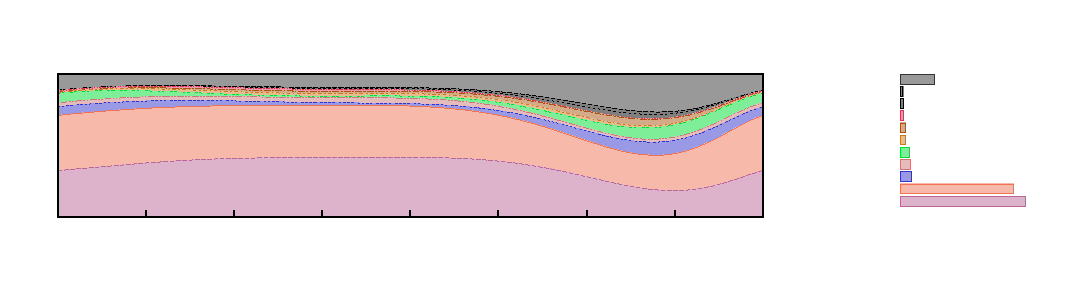
\includegraphics{img/in}}%
    \gplfronttext
  \end{picture}%
\endgroup


\noindent% GNUPLOT: LaTeX picture with Postscript
\begingroup
  \makeatletter
  \providecommand\color[2][]{%
    \GenericError{(gnuplot) \space\space\space\@spaces}{%
      Package color not loaded in conjunction with
      terminal option `colourtext'%
    }{See the gnuplot documentation for explanation.%
    }{Either use 'blacktext' in gnuplot or load the package
      color.sty in LaTeX.}%
    \renewcommand\color[2][]{}%
  }%
  \providecommand\includegraphics[2][]{%
    \GenericError{(gnuplot) \space\space\space\@spaces}{%
      Package graphicx or graphics not loaded%
    }{See the gnuplot documentation for explanation.%
    }{The gnuplot epslatex terminal needs graphicx.sty or graphics.sty.}%
    \renewcommand\includegraphics[2][]{}%
  }%
  \providecommand\rotatebox[2]{#2}%
  \@ifundefined{ifGPcolor}{%
    \newif\ifGPcolor
    \GPcolorfalse
  }{}%
  \@ifundefined{ifGPblacktext}{%
    \newif\ifGPblacktext
    \GPblacktexttrue
  }{}%
  % define a \g@addto@macro without @ in the name:
  \let\gplgaddtomacro\g@addto@macro
  % define empty templates for all commands taking text:
  \gdef\gplbacktext{}%
  \gdef\gplfronttext{}%
  \makeatother
  \ifGPblacktext
    % no textcolor at all
    \def\colorrgb#1{}%
    \def\colorgray#1{}%
  \else
    % gray or color?
    \ifGPcolor
      \def\colorrgb#1{\color[rgb]{#1}}%
      \def\colorgray#1{\color[gray]{#1}}%
      \expandafter\def\csname LTw\endcsname{\color{white}}%
      \expandafter\def\csname LTb\endcsname{\color{black}}%
      \expandafter\def\csname LTa\endcsname{\color{black}}%
      \expandafter\def\csname LT0\endcsname{\color[rgb]{1,0,0}}%
      \expandafter\def\csname LT1\endcsname{\color[rgb]{0,1,0}}%
      \expandafter\def\csname LT2\endcsname{\color[rgb]{0,0,1}}%
      \expandafter\def\csname LT3\endcsname{\color[rgb]{1,0,1}}%
      \expandafter\def\csname LT4\endcsname{\color[rgb]{0,1,1}}%
      \expandafter\def\csname LT5\endcsname{\color[rgb]{1,1,0}}%
      \expandafter\def\csname LT6\endcsname{\color[rgb]{0,0,0}}%
      \expandafter\def\csname LT7\endcsname{\color[rgb]{1,0.3,0}}%
      \expandafter\def\csname LT8\endcsname{\color[rgb]{0.5,0.5,0.5}}%
    \else
      % gray
      \def\colorrgb#1{\color{black}}%
      \def\colorgray#1{\color[gray]{#1}}%
      \expandafter\def\csname LTw\endcsname{\color{white}}%
      \expandafter\def\csname LTb\endcsname{\color{black}}%
      \expandafter\def\csname LTa\endcsname{\color{black}}%
      \expandafter\def\csname LT0\endcsname{\color{black}}%
      \expandafter\def\csname LT1\endcsname{\color{black}}%
      \expandafter\def\csname LT2\endcsname{\color{black}}%
      \expandafter\def\csname LT3\endcsname{\color{black}}%
      \expandafter\def\csname LT4\endcsname{\color{black}}%
      \expandafter\def\csname LT5\endcsname{\color{black}}%
      \expandafter\def\csname LT6\endcsname{\color{black}}%
      \expandafter\def\csname LT7\endcsname{\color{black}}%
      \expandafter\def\csname LT8\endcsname{\color{black}}%
    \fi
  \fi
  \setlength{\unitlength}{0.0500bp}%
  \begin{picture}(10080.00,2520.00)%
    \gplgaddtomacro\gplbacktext{%
      \csname LTb\endcsname%
      \put(176,1281){\rotatebox{-270}{\makebox(0,0){\strut{}\scriptsize fraction of tweets}}}%
      \put(3779,154){\makebox(0,0){\strut{}\scriptsize time of day (UTC)}}%
      \put(3779,2189){\makebox(0,0){\strut{}Countries that Tweet in Tagalog}}%
    }%
    \gplgaddtomacro\gplfronttext{%
      \csname LTb\endcsname%
      \put(396,374){\makebox(0,0){\strut{}\scriptsize 0:00}}%
      \put(1242,374){\makebox(0,0){\strut{}\scriptsize 3:00}}%
      \put(2088,374){\makebox(0,0){\strut{}\scriptsize 6:00}}%
      \put(2934,374){\makebox(0,0){\strut{}\scriptsize 9:00}}%
      \put(3780,374){\makebox(0,0){\strut{}\scriptsize 12:00}}%
      \put(4625,374){\makebox(0,0){\strut{}\scriptsize 15:00}}%
      \put(5471,374){\makebox(0,0){\strut{}\scriptsize 18:00}}%
      \put(6317,374){\makebox(0,0){\strut{}\scriptsize 21:00}}%
      \put(7163,374){\makebox(0,0){\strut{}\scriptsize 24:00}}%
    }%
    \gplgaddtomacro\gplbacktext{%
      \csname LTb\endcsname%
      \put(9083,154){\makebox(0,0){\strut{}~~}}%
      \put(9083,2189){\makebox(0,0){\strut{} }}%
    }%
    \gplgaddtomacro\gplfronttext{%
      \csname LTb\endcsname%
      \put(8352,751){\makebox(0,0)[r]{\strut{}\scriptsize~Philippines}}%
      \put(8352,868){\makebox(0,0)[r]{\strut{}\scriptsize~USA}}%
      \put(8352,985){\makebox(0,0)[r]{\strut{}\scriptsize~Malasia}}%
      \put(8352,1102){\makebox(0,0)[r]{\strut{}\scriptsize~Brazil}}%
      \put(8352,1219){\makebox(0,0)[r]{\strut{}\scriptsize~South~Africa}}%
      \put(8352,1337){\makebox(0,0)[r]{\strut{}\scriptsize~Indonesia}}%
      \put(8352,1454){\makebox(0,0)[r]{\strut{}\scriptsize~UK}}%
      \put(8352,1571){\makebox(0,0)[r]{\strut{}\scriptsize~India}}%
      \put(8352,1688){\makebox(0,0)[r]{\strut{}\scriptsize~Canada}}%
      \put(8352,1805){\makebox(0,0)[r]{\strut{}\scriptsize~Arab~Emirates}}%
      \put(8352,1922){\makebox(0,0)[r]{\strut{}\scriptsize~other}}%
    }%
    \gplbacktext
    \put(0,0){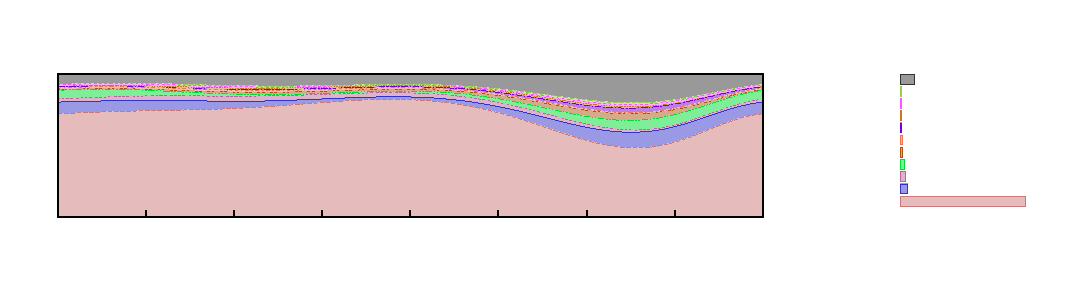
\includegraphics{img/tl}}%
    \gplfronttext
  \end{picture}%
\endgroup


\noindent% GNUPLOT: LaTeX picture with Postscript
\begingroup
  \makeatletter
  \providecommand\color[2][]{%
    \GenericError{(gnuplot) \space\space\space\@spaces}{%
      Package color not loaded in conjunction with
      terminal option `colourtext'%
    }{See the gnuplot documentation for explanation.%
    }{Either use 'blacktext' in gnuplot or load the package
      color.sty in LaTeX.}%
    \renewcommand\color[2][]{}%
  }%
  \providecommand\includegraphics[2][]{%
    \GenericError{(gnuplot) \space\space\space\@spaces}{%
      Package graphicx or graphics not loaded%
    }{See the gnuplot documentation for explanation.%
    }{The gnuplot epslatex terminal needs graphicx.sty or graphics.sty.}%
    \renewcommand\includegraphics[2][]{}%
  }%
  \providecommand\rotatebox[2]{#2}%
  \@ifundefined{ifGPcolor}{%
    \newif\ifGPcolor
    \GPcolorfalse
  }{}%
  \@ifundefined{ifGPblacktext}{%
    \newif\ifGPblacktext
    \GPblacktexttrue
  }{}%
  % define a \g@addto@macro without @ in the name:
  \let\gplgaddtomacro\g@addto@macro
  % define empty templates for all commands taking text:
  \gdef\gplbacktext{}%
  \gdef\gplfronttext{}%
  \makeatother
  \ifGPblacktext
    % no textcolor at all
    \def\colorrgb#1{}%
    \def\colorgray#1{}%
  \else
    % gray or color?
    \ifGPcolor
      \def\colorrgb#1{\color[rgb]{#1}}%
      \def\colorgray#1{\color[gray]{#1}}%
      \expandafter\def\csname LTw\endcsname{\color{white}}%
      \expandafter\def\csname LTb\endcsname{\color{black}}%
      \expandafter\def\csname LTa\endcsname{\color{black}}%
      \expandafter\def\csname LT0\endcsname{\color[rgb]{1,0,0}}%
      \expandafter\def\csname LT1\endcsname{\color[rgb]{0,1,0}}%
      \expandafter\def\csname LT2\endcsname{\color[rgb]{0,0,1}}%
      \expandafter\def\csname LT3\endcsname{\color[rgb]{1,0,1}}%
      \expandafter\def\csname LT4\endcsname{\color[rgb]{0,1,1}}%
      \expandafter\def\csname LT5\endcsname{\color[rgb]{1,1,0}}%
      \expandafter\def\csname LT6\endcsname{\color[rgb]{0,0,0}}%
      \expandafter\def\csname LT7\endcsname{\color[rgb]{1,0.3,0}}%
      \expandafter\def\csname LT8\endcsname{\color[rgb]{0.5,0.5,0.5}}%
    \else
      % gray
      \def\colorrgb#1{\color{black}}%
      \def\colorgray#1{\color[gray]{#1}}%
      \expandafter\def\csname LTw\endcsname{\color{white}}%
      \expandafter\def\csname LTb\endcsname{\color{black}}%
      \expandafter\def\csname LTa\endcsname{\color{black}}%
      \expandafter\def\csname LT0\endcsname{\color{black}}%
      \expandafter\def\csname LT1\endcsname{\color{black}}%
      \expandafter\def\csname LT2\endcsname{\color{black}}%
      \expandafter\def\csname LT3\endcsname{\color{black}}%
      \expandafter\def\csname LT4\endcsname{\color{black}}%
      \expandafter\def\csname LT5\endcsname{\color{black}}%
      \expandafter\def\csname LT6\endcsname{\color{black}}%
      \expandafter\def\csname LT7\endcsname{\color{black}}%
      \expandafter\def\csname LT8\endcsname{\color{black}}%
    \fi
  \fi
  \setlength{\unitlength}{0.0500bp}%
  \begin{picture}(10080.00,2520.00)%
    \gplgaddtomacro\gplbacktext{%
      \csname LTb\endcsname%
      \put(176,1281){\rotatebox{-270}{\makebox(0,0){\strut{}\scriptsize fraction of tweets}}}%
      \put(3779,154){\makebox(0,0){\strut{}\scriptsize time of day (UTC)}}%
      \put(3779,2189){\makebox(0,0){\strut{}Countries that Tweet in Turkish}}%
    }%
    \gplgaddtomacro\gplfronttext{%
      \csname LTb\endcsname%
      \put(396,374){\makebox(0,0){\strut{}\scriptsize 0:00}}%
      \put(1242,374){\makebox(0,0){\strut{}\scriptsize 3:00}}%
      \put(2088,374){\makebox(0,0){\strut{}\scriptsize 6:00}}%
      \put(2934,374){\makebox(0,0){\strut{}\scriptsize 9:00}}%
      \put(3780,374){\makebox(0,0){\strut{}\scriptsize 12:00}}%
      \put(4625,374){\makebox(0,0){\strut{}\scriptsize 15:00}}%
      \put(5471,374){\makebox(0,0){\strut{}\scriptsize 18:00}}%
      \put(6317,374){\makebox(0,0){\strut{}\scriptsize 21:00}}%
      \put(7163,374){\makebox(0,0){\strut{}\scriptsize 24:00}}%
    }%
    \gplgaddtomacro\gplbacktext{%
      \csname LTb\endcsname%
      \put(9083,154){\makebox(0,0){\strut{}~~}}%
      \put(9083,2189){\makebox(0,0){\strut{} }}%
    }%
    \gplgaddtomacro\gplfronttext{%
      \csname LTb\endcsname%
      \put(8352,751){\makebox(0,0)[r]{\strut{}\scriptsize~TR}}%
      \put(8352,868){\makebox(0,0)[r]{\strut{}\scriptsize~USA}}%
      \put(8352,985){\makebox(0,0)[r]{\strut{}\scriptsize~geo}}%
      \put(8352,1102){\makebox(0,0)[r]{\strut{}\scriptsize~DE}}%
      \put(8352,1219){\makebox(0,0)[r]{\strut{}\scriptsize~Brazil}}%
      \put(8352,1337){\makebox(0,0)[r]{\strut{}\scriptsize~CY}}%
      \put(8352,1454){\makebox(0,0)[r]{\strut{}\scriptsize~AZ}}%
      \put(8352,1571){\makebox(0,0)[r]{\strut{}\scriptsize~blank}}%
      \put(8352,1688){\makebox(0,0)[r]{\strut{}\scriptsize~France}}%
      \put(8352,1805){\makebox(0,0)[r]{\strut{}\scriptsize~Philippines}}%
      \put(8352,1922){\makebox(0,0)[r]{\strut{}\scriptsize~other}}%
    }%
    \gplbacktext
    \put(0,0){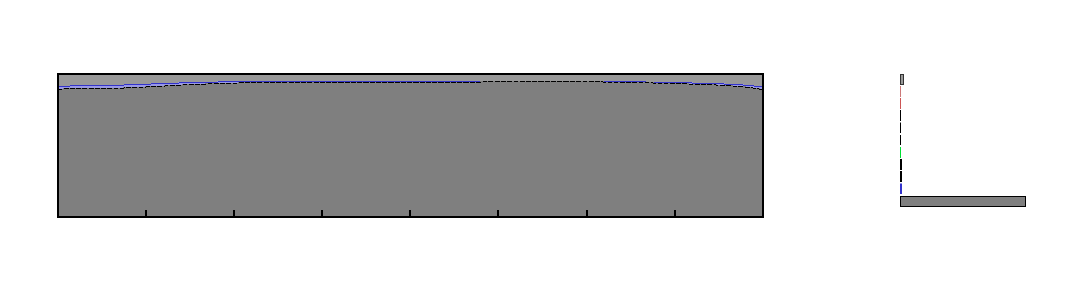
\includegraphics{img/tr}}%
    \gplfronttext
  \end{picture}%
\endgroup


\noindent% GNUPLOT: LaTeX picture with Postscript
\begingroup
  \makeatletter
  \providecommand\color[2][]{%
    \GenericError{(gnuplot) \space\space\space\@spaces}{%
      Package color not loaded in conjunction with
      terminal option `colourtext'%
    }{See the gnuplot documentation for explanation.%
    }{Either use 'blacktext' in gnuplot or load the package
      color.sty in LaTeX.}%
    \renewcommand\color[2][]{}%
  }%
  \providecommand\includegraphics[2][]{%
    \GenericError{(gnuplot) \space\space\space\@spaces}{%
      Package graphicx or graphics not loaded%
    }{See the gnuplot documentation for explanation.%
    }{The gnuplot epslatex terminal needs graphicx.sty or graphics.sty.}%
    \renewcommand\includegraphics[2][]{}%
  }%
  \providecommand\rotatebox[2]{#2}%
  \@ifundefined{ifGPcolor}{%
    \newif\ifGPcolor
    \GPcolorfalse
  }{}%
  \@ifundefined{ifGPblacktext}{%
    \newif\ifGPblacktext
    \GPblacktexttrue
  }{}%
  % define a \g@addto@macro without @ in the name:
  \let\gplgaddtomacro\g@addto@macro
  % define empty templates for all commands taking text:
  \gdef\gplbacktext{}%
  \gdef\gplfronttext{}%
  \makeatother
  \ifGPblacktext
    % no textcolor at all
    \def\colorrgb#1{}%
    \def\colorgray#1{}%
  \else
    % gray or color?
    \ifGPcolor
      \def\colorrgb#1{\color[rgb]{#1}}%
      \def\colorgray#1{\color[gray]{#1}}%
      \expandafter\def\csname LTw\endcsname{\color{white}}%
      \expandafter\def\csname LTb\endcsname{\color{black}}%
      \expandafter\def\csname LTa\endcsname{\color{black}}%
      \expandafter\def\csname LT0\endcsname{\color[rgb]{1,0,0}}%
      \expandafter\def\csname LT1\endcsname{\color[rgb]{0,1,0}}%
      \expandafter\def\csname LT2\endcsname{\color[rgb]{0,0,1}}%
      \expandafter\def\csname LT3\endcsname{\color[rgb]{1,0,1}}%
      \expandafter\def\csname LT4\endcsname{\color[rgb]{0,1,1}}%
      \expandafter\def\csname LT5\endcsname{\color[rgb]{1,1,0}}%
      \expandafter\def\csname LT6\endcsname{\color[rgb]{0,0,0}}%
      \expandafter\def\csname LT7\endcsname{\color[rgb]{1,0.3,0}}%
      \expandafter\def\csname LT8\endcsname{\color[rgb]{0.5,0.5,0.5}}%
    \else
      % gray
      \def\colorrgb#1{\color{black}}%
      \def\colorgray#1{\color[gray]{#1}}%
      \expandafter\def\csname LTw\endcsname{\color{white}}%
      \expandafter\def\csname LTb\endcsname{\color{black}}%
      \expandafter\def\csname LTa\endcsname{\color{black}}%
      \expandafter\def\csname LT0\endcsname{\color{black}}%
      \expandafter\def\csname LT1\endcsname{\color{black}}%
      \expandafter\def\csname LT2\endcsname{\color{black}}%
      \expandafter\def\csname LT3\endcsname{\color{black}}%
      \expandafter\def\csname LT4\endcsname{\color{black}}%
      \expandafter\def\csname LT5\endcsname{\color{black}}%
      \expandafter\def\csname LT6\endcsname{\color{black}}%
      \expandafter\def\csname LT7\endcsname{\color{black}}%
      \expandafter\def\csname LT8\endcsname{\color{black}}%
    \fi
  \fi
  \setlength{\unitlength}{0.0500bp}%
  \begin{picture}(10080.00,2520.00)%
    \gplgaddtomacro\gplbacktext{%
      \csname LTb\endcsname%
      \put(176,1281){\rotatebox{-270}{\makebox(0,0){\strut{}\scriptsize fraction of tweets}}}%
      \put(3779,154){\makebox(0,0){\strut{}\scriptsize time of day (UTC)}}%
      \put(3779,2189){\makebox(0,0){\strut{}Countries that Tweet in Japanese}}%
    }%
    \gplgaddtomacro\gplfronttext{%
      \csname LTb\endcsname%
      \put(396,374){\makebox(0,0){\strut{}\scriptsize 0:00}}%
      \put(1242,374){\makebox(0,0){\strut{}\scriptsize 3:00}}%
      \put(2088,374){\makebox(0,0){\strut{}\scriptsize 6:00}}%
      \put(2934,374){\makebox(0,0){\strut{}\scriptsize 9:00}}%
      \put(3780,374){\makebox(0,0){\strut{}\scriptsize 12:00}}%
      \put(4625,374){\makebox(0,0){\strut{}\scriptsize 15:00}}%
      \put(5471,374){\makebox(0,0){\strut{}\scriptsize 18:00}}%
      \put(6317,374){\makebox(0,0){\strut{}\scriptsize 21:00}}%
      \put(7163,374){\makebox(0,0){\strut{}\scriptsize 24:00}}%
    }%
    \gplgaddtomacro\gplbacktext{%
      \csname LTb\endcsname%
      \put(9083,154){\makebox(0,0){\strut{}~~}}%
      \put(9083,2189){\makebox(0,0){\strut{} }}%
    }%
    \gplgaddtomacro\gplfronttext{%
      \csname LTb\endcsname%
      \put(8352,751){\makebox(0,0)[r]{\strut{}\scriptsize~Japan}}%
      \put(8352,868){\makebox(0,0)[r]{\strut{}\scriptsize~USA}}%
      \put(8352,985){\makebox(0,0)[r]{\strut{}\scriptsize~Taiwan}}%
      \put(8352,1102){\makebox(0,0)[r]{\strut{}\scriptsize~China}}%
      \put(8352,1219){\makebox(0,0)[r]{\strut{}\scriptsize~Thailand}}%
      \put(8352,1337){\makebox(0,0)[r]{\strut{}\scriptsize~South~Korea}}%
      \put(8352,1454){\makebox(0,0)[r]{\strut{}\scriptsize~Australia}}%
      \put(8352,1571){\makebox(0,0)[r]{\strut{}\scriptsize~Hong~Kong}}%
      \put(8352,1688){\makebox(0,0)[r]{\strut{}\scriptsize~Malasia}}%
      \put(8352,1805){\makebox(0,0)[r]{\strut{}\scriptsize~geo}}%
      \put(8352,1922){\makebox(0,0)[r]{\strut{}\scriptsize~other}}%
    }%
    \gplbacktext
    \put(0,0){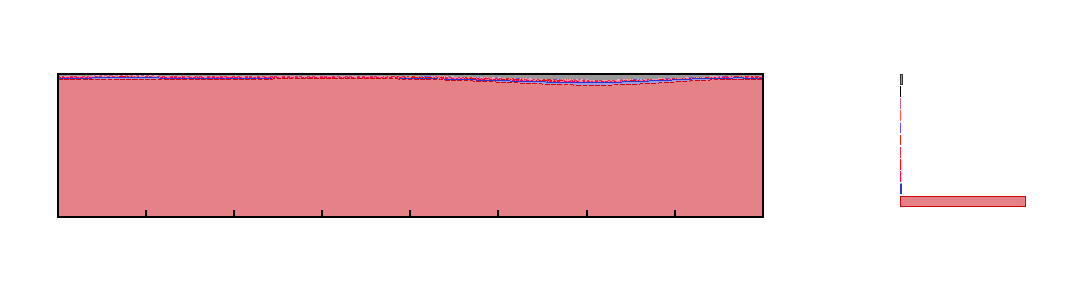
\includegraphics{img/ja}}%
    \gplfronttext
  \end{picture}%
\endgroup


\noindent% GNUPLOT: LaTeX picture with Postscript
\begingroup
  \makeatletter
  \providecommand\color[2][]{%
    \GenericError{(gnuplot) \space\space\space\@spaces}{%
      Package color not loaded in conjunction with
      terminal option `colourtext'%
    }{See the gnuplot documentation for explanation.%
    }{Either use 'blacktext' in gnuplot or load the package
      color.sty in LaTeX.}%
    \renewcommand\color[2][]{}%
  }%
  \providecommand\includegraphics[2][]{%
    \GenericError{(gnuplot) \space\space\space\@spaces}{%
      Package graphicx or graphics not loaded%
    }{See the gnuplot documentation for explanation.%
    }{The gnuplot epslatex terminal needs graphicx.sty or graphics.sty.}%
    \renewcommand\includegraphics[2][]{}%
  }%
  \providecommand\rotatebox[2]{#2}%
  \@ifundefined{ifGPcolor}{%
    \newif\ifGPcolor
    \GPcolorfalse
  }{}%
  \@ifundefined{ifGPblacktext}{%
    \newif\ifGPblacktext
    \GPblacktexttrue
  }{}%
  % define a \g@addto@macro without @ in the name:
  \let\gplgaddtomacro\g@addto@macro
  % define empty templates for all commands taking text:
  \gdef\gplbacktext{}%
  \gdef\gplfronttext{}%
  \makeatother
  \ifGPblacktext
    % no textcolor at all
    \def\colorrgb#1{}%
    \def\colorgray#1{}%
  \else
    % gray or color?
    \ifGPcolor
      \def\colorrgb#1{\color[rgb]{#1}}%
      \def\colorgray#1{\color[gray]{#1}}%
      \expandafter\def\csname LTw\endcsname{\color{white}}%
      \expandafter\def\csname LTb\endcsname{\color{black}}%
      \expandafter\def\csname LTa\endcsname{\color{black}}%
      \expandafter\def\csname LT0\endcsname{\color[rgb]{1,0,0}}%
      \expandafter\def\csname LT1\endcsname{\color[rgb]{0,1,0}}%
      \expandafter\def\csname LT2\endcsname{\color[rgb]{0,0,1}}%
      \expandafter\def\csname LT3\endcsname{\color[rgb]{1,0,1}}%
      \expandafter\def\csname LT4\endcsname{\color[rgb]{0,1,1}}%
      \expandafter\def\csname LT5\endcsname{\color[rgb]{1,1,0}}%
      \expandafter\def\csname LT6\endcsname{\color[rgb]{0,0,0}}%
      \expandafter\def\csname LT7\endcsname{\color[rgb]{1,0.3,0}}%
      \expandafter\def\csname LT8\endcsname{\color[rgb]{0.5,0.5,0.5}}%
    \else
      % gray
      \def\colorrgb#1{\color{black}}%
      \def\colorgray#1{\color[gray]{#1}}%
      \expandafter\def\csname LTw\endcsname{\color{white}}%
      \expandafter\def\csname LTb\endcsname{\color{black}}%
      \expandafter\def\csname LTa\endcsname{\color{black}}%
      \expandafter\def\csname LT0\endcsname{\color{black}}%
      \expandafter\def\csname LT1\endcsname{\color{black}}%
      \expandafter\def\csname LT2\endcsname{\color{black}}%
      \expandafter\def\csname LT3\endcsname{\color{black}}%
      \expandafter\def\csname LT4\endcsname{\color{black}}%
      \expandafter\def\csname LT5\endcsname{\color{black}}%
      \expandafter\def\csname LT6\endcsname{\color{black}}%
      \expandafter\def\csname LT7\endcsname{\color{black}}%
      \expandafter\def\csname LT8\endcsname{\color{black}}%
    \fi
  \fi
  \setlength{\unitlength}{0.0500bp}%
  \begin{picture}(10080.00,2520.00)%
    \gplgaddtomacro\gplbacktext{%
      \csname LTb\endcsname%
      \put(176,1281){\rotatebox{-270}{\makebox(0,0){\strut{}\scriptsize fraction of tweets}}}%
      \put(3779,154){\makebox(0,0){\strut{}\scriptsize time of day (UTC)}}%
      \put(3779,2189){\makebox(0,0){\strut{}Countries that Tweet in ko}}%
    }%
    \gplgaddtomacro\gplfronttext{%
      \csname LTb\endcsname%
      \put(396,374){\makebox(0,0){\strut{}\scriptsize 0:00}}%
      \put(1242,374){\makebox(0,0){\strut{}\scriptsize 3:00}}%
      \put(2088,374){\makebox(0,0){\strut{}\scriptsize 6:00}}%
      \put(2934,374){\makebox(0,0){\strut{}\scriptsize 9:00}}%
      \put(3780,374){\makebox(0,0){\strut{}\scriptsize 12:00}}%
      \put(4625,374){\makebox(0,0){\strut{}\scriptsize 15:00}}%
      \put(5471,374){\makebox(0,0){\strut{}\scriptsize 18:00}}%
      \put(6317,374){\makebox(0,0){\strut{}\scriptsize 21:00}}%
      \put(7163,374){\makebox(0,0){\strut{}\scriptsize 24:00}}%
    }%
    \gplgaddtomacro\gplbacktext{%
      \csname LTb\endcsname%
      \put(9083,154){\makebox(0,0){\strut{}~~}}%
      \put(9083,2189){\makebox(0,0){\strut{} }}%
    }%
    \gplgaddtomacro\gplfronttext{%
      \csname LTb\endcsname%
      \put(8352,751){\makebox(0,0)[r]{\strut{}\scriptsize~South~Korea}}%
      \put(8352,868){\makebox(0,0)[r]{\strut{}\scriptsize~Japan}}%
      \put(8352,985){\makebox(0,0)[r]{\strut{}\scriptsize~USA}}%
      \put(8352,1102){\makebox(0,0)[r]{\strut{}\scriptsize~Thailand}}%
      \put(8352,1219){\makebox(0,0)[r]{\strut{}\scriptsize~Russia}}%
      \put(8352,1337){\makebox(0,0)[r]{\strut{}\scriptsize~Indonesia}}%
      \put(8352,1454){\makebox(0,0)[r]{\strut{}\scriptsize~Philippines}}%
      \put(8352,1571){\makebox(0,0)[r]{\strut{}\scriptsize~Brazil}}%
      \put(8352,1688){\makebox(0,0)[r]{\strut{}\scriptsize~Australia}}%
      \put(8352,1805){\makebox(0,0)[r]{\strut{}\scriptsize~Malasia}}%
      \put(8352,1922){\makebox(0,0)[r]{\strut{}\scriptsize~other}}%
    }%
    \gplbacktext
    \put(0,0){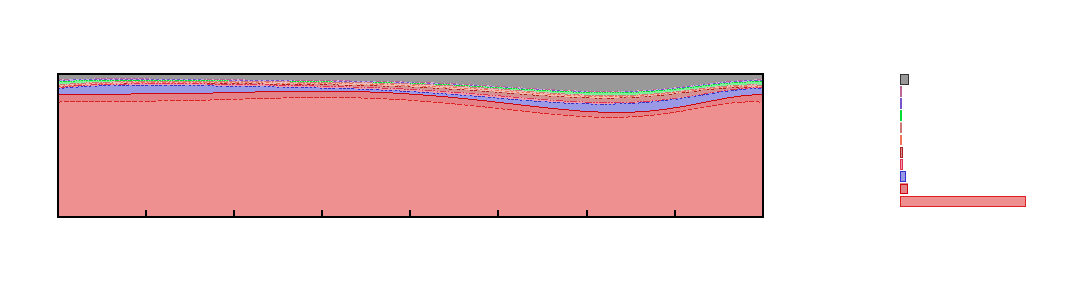
\includegraphics{img/ko}}%
    \gplfronttext
  \end{picture}%
\endgroup


\noindent% GNUPLOT: LaTeX picture with Postscript
\begingroup
  \makeatletter
  \providecommand\color[2][]{%
    \GenericError{(gnuplot) \space\space\space\@spaces}{%
      Package color not loaded in conjunction with
      terminal option `colourtext'%
    }{See the gnuplot documentation for explanation.%
    }{Either use 'blacktext' in gnuplot or load the package
      color.sty in LaTeX.}%
    \renewcommand\color[2][]{}%
  }%
  \providecommand\includegraphics[2][]{%
    \GenericError{(gnuplot) \space\space\space\@spaces}{%
      Package graphicx or graphics not loaded%
    }{See the gnuplot documentation for explanation.%
    }{The gnuplot epslatex terminal needs graphicx.sty or graphics.sty.}%
    \renewcommand\includegraphics[2][]{}%
  }%
  \providecommand\rotatebox[2]{#2}%
  \@ifundefined{ifGPcolor}{%
    \newif\ifGPcolor
    \GPcolorfalse
  }{}%
  \@ifundefined{ifGPblacktext}{%
    \newif\ifGPblacktext
    \GPblacktexttrue
  }{}%
  % define a \g@addto@macro without @ in the name:
  \let\gplgaddtomacro\g@addto@macro
  % define empty templates for all commands taking text:
  \gdef\gplbacktext{}%
  \gdef\gplfronttext{}%
  \makeatother
  \ifGPblacktext
    % no textcolor at all
    \def\colorrgb#1{}%
    \def\colorgray#1{}%
  \else
    % gray or color?
    \ifGPcolor
      \def\colorrgb#1{\color[rgb]{#1}}%
      \def\colorgray#1{\color[gray]{#1}}%
      \expandafter\def\csname LTw\endcsname{\color{white}}%
      \expandafter\def\csname LTb\endcsname{\color{black}}%
      \expandafter\def\csname LTa\endcsname{\color{black}}%
      \expandafter\def\csname LT0\endcsname{\color[rgb]{1,0,0}}%
      \expandafter\def\csname LT1\endcsname{\color[rgb]{0,1,0}}%
      \expandafter\def\csname LT2\endcsname{\color[rgb]{0,0,1}}%
      \expandafter\def\csname LT3\endcsname{\color[rgb]{1,0,1}}%
      \expandafter\def\csname LT4\endcsname{\color[rgb]{0,1,1}}%
      \expandafter\def\csname LT5\endcsname{\color[rgb]{1,1,0}}%
      \expandafter\def\csname LT6\endcsname{\color[rgb]{0,0,0}}%
      \expandafter\def\csname LT7\endcsname{\color[rgb]{1,0.3,0}}%
      \expandafter\def\csname LT8\endcsname{\color[rgb]{0.5,0.5,0.5}}%
    \else
      % gray
      \def\colorrgb#1{\color{black}}%
      \def\colorgray#1{\color[gray]{#1}}%
      \expandafter\def\csname LTw\endcsname{\color{white}}%
      \expandafter\def\csname LTb\endcsname{\color{black}}%
      \expandafter\def\csname LTa\endcsname{\color{black}}%
      \expandafter\def\csname LT0\endcsname{\color{black}}%
      \expandafter\def\csname LT1\endcsname{\color{black}}%
      \expandafter\def\csname LT2\endcsname{\color{black}}%
      \expandafter\def\csname LT3\endcsname{\color{black}}%
      \expandafter\def\csname LT4\endcsname{\color{black}}%
      \expandafter\def\csname LT5\endcsname{\color{black}}%
      \expandafter\def\csname LT6\endcsname{\color{black}}%
      \expandafter\def\csname LT7\endcsname{\color{black}}%
      \expandafter\def\csname LT8\endcsname{\color{black}}%
    \fi
  \fi
  \setlength{\unitlength}{0.0500bp}%
  \begin{picture}(10080.00,2520.00)%
    \gplgaddtomacro\gplbacktext{%
      \csname LTb\endcsname%
      \put(176,1281){\rotatebox{-270}{\makebox(0,0){\strut{}\scriptsize fraction of tweets}}}%
      \put(3779,154){\makebox(0,0){\strut{}\scriptsize time of day (UTC)}}%
      \put(3779,2189){\makebox(0,0){\strut{}Countries that Tweet in Portuguese}}%
    }%
    \gplgaddtomacro\gplfronttext{%
      \csname LTb\endcsname%
      \put(396,374){\makebox(0,0){\strut{}\scriptsize 0:00}}%
      \put(1242,374){\makebox(0,0){\strut{}\scriptsize 3:00}}%
      \put(2088,374){\makebox(0,0){\strut{}\scriptsize 6:00}}%
      \put(2934,374){\makebox(0,0){\strut{}\scriptsize 9:00}}%
      \put(3780,374){\makebox(0,0){\strut{}\scriptsize 12:00}}%
      \put(4625,374){\makebox(0,0){\strut{}\scriptsize 15:00}}%
      \put(5471,374){\makebox(0,0){\strut{}\scriptsize 18:00}}%
      \put(6317,374){\makebox(0,0){\strut{}\scriptsize 21:00}}%
      \put(7163,374){\makebox(0,0){\strut{}\scriptsize 24:00}}%
    }%
    \gplgaddtomacro\gplbacktext{%
      \csname LTb\endcsname%
      \put(9083,154){\makebox(0,0){\strut{}~~}}%
      \put(9083,2189){\makebox(0,0){\strut{} }}%
    }%
    \gplgaddtomacro\gplfronttext{%
      \csname LTb\endcsname%
      \put(8352,751){\makebox(0,0)[r]{\strut{}\scriptsize~Brazil}}%
      \put(8352,868){\makebox(0,0)[r]{\strut{}\scriptsize~Portugal}}%
      \put(8352,985){\makebox(0,0)[r]{\strut{}\scriptsize~USA}}%
      \put(8352,1102){\makebox(0,0)[r]{\strut{}\scriptsize~Argentina}}%
      \put(8352,1219){\makebox(0,0)[r]{\strut{}\scriptsize~Spain}}%
      \put(8352,1337){\makebox(0,0)[r]{\strut{}\scriptsize~Mexico}}%
      \put(8352,1454){\makebox(0,0)[r]{\strut{}\scriptsize~UK}}%
      \put(8352,1571){\makebox(0,0)[r]{\strut{}\scriptsize~France}}%
      \put(8352,1688){\makebox(0,0)[r]{\strut{}\scriptsize~Italy}}%
      \put(8352,1805){\makebox(0,0)[r]{\strut{}\scriptsize~Canada}}%
      \put(8352,1922){\makebox(0,0)[r]{\strut{}\scriptsize~other}}%
    }%
    \gplbacktext
    \put(0,0){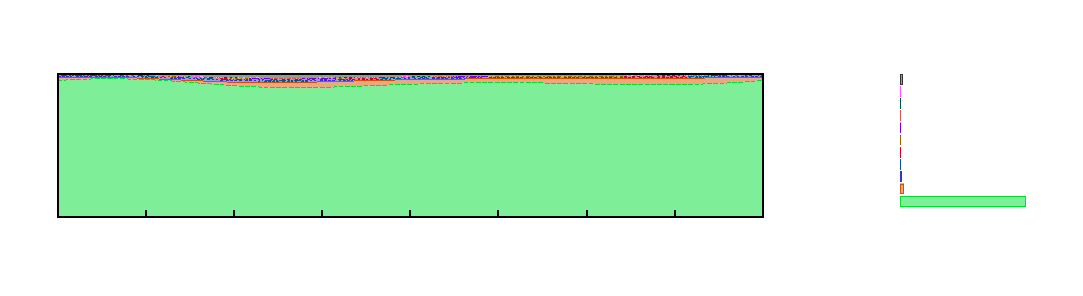
\includegraphics{img/pt}}%
    \gplfronttext
  \end{picture}%
\endgroup


\noindent% GNUPLOT: LaTeX picture with Postscript
\begingroup
  \makeatletter
  \providecommand\color[2][]{%
    \GenericError{(gnuplot) \space\space\space\@spaces}{%
      Package color not loaded in conjunction with
      terminal option `colourtext'%
    }{See the gnuplot documentation for explanation.%
    }{Either use 'blacktext' in gnuplot or load the package
      color.sty in LaTeX.}%
    \renewcommand\color[2][]{}%
  }%
  \providecommand\includegraphics[2][]{%
    \GenericError{(gnuplot) \space\space\space\@spaces}{%
      Package graphicx or graphics not loaded%
    }{See the gnuplot documentation for explanation.%
    }{The gnuplot epslatex terminal needs graphicx.sty or graphics.sty.}%
    \renewcommand\includegraphics[2][]{}%
  }%
  \providecommand\rotatebox[2]{#2}%
  \@ifundefined{ifGPcolor}{%
    \newif\ifGPcolor
    \GPcolorfalse
  }{}%
  \@ifundefined{ifGPblacktext}{%
    \newif\ifGPblacktext
    \GPblacktexttrue
  }{}%
  % define a \g@addto@macro without @ in the name:
  \let\gplgaddtomacro\g@addto@macro
  % define empty templates for all commands taking text:
  \gdef\gplbacktext{}%
  \gdef\gplfronttext{}%
  \makeatother
  \ifGPblacktext
    % no textcolor at all
    \def\colorrgb#1{}%
    \def\colorgray#1{}%
  \else
    % gray or color?
    \ifGPcolor
      \def\colorrgb#1{\color[rgb]{#1}}%
      \def\colorgray#1{\color[gray]{#1}}%
      \expandafter\def\csname LTw\endcsname{\color{white}}%
      \expandafter\def\csname LTb\endcsname{\color{black}}%
      \expandafter\def\csname LTa\endcsname{\color{black}}%
      \expandafter\def\csname LT0\endcsname{\color[rgb]{1,0,0}}%
      \expandafter\def\csname LT1\endcsname{\color[rgb]{0,1,0}}%
      \expandafter\def\csname LT2\endcsname{\color[rgb]{0,0,1}}%
      \expandafter\def\csname LT3\endcsname{\color[rgb]{1,0,1}}%
      \expandafter\def\csname LT4\endcsname{\color[rgb]{0,1,1}}%
      \expandafter\def\csname LT5\endcsname{\color[rgb]{1,1,0}}%
      \expandafter\def\csname LT6\endcsname{\color[rgb]{0,0,0}}%
      \expandafter\def\csname LT7\endcsname{\color[rgb]{1,0.3,0}}%
      \expandafter\def\csname LT8\endcsname{\color[rgb]{0.5,0.5,0.5}}%
    \else
      % gray
      \def\colorrgb#1{\color{black}}%
      \def\colorgray#1{\color[gray]{#1}}%
      \expandafter\def\csname LTw\endcsname{\color{white}}%
      \expandafter\def\csname LTb\endcsname{\color{black}}%
      \expandafter\def\csname LTa\endcsname{\color{black}}%
      \expandafter\def\csname LT0\endcsname{\color{black}}%
      \expandafter\def\csname LT1\endcsname{\color{black}}%
      \expandafter\def\csname LT2\endcsname{\color{black}}%
      \expandafter\def\csname LT3\endcsname{\color{black}}%
      \expandafter\def\csname LT4\endcsname{\color{black}}%
      \expandafter\def\csname LT5\endcsname{\color{black}}%
      \expandafter\def\csname LT6\endcsname{\color{black}}%
      \expandafter\def\csname LT7\endcsname{\color{black}}%
      \expandafter\def\csname LT8\endcsname{\color{black}}%
    \fi
  \fi
  \setlength{\unitlength}{0.0500bp}%
  \begin{picture}(10080.00,2520.00)%
    \gplgaddtomacro\gplbacktext{%
      \csname LTb\endcsname%
      \put(176,1281){\rotatebox{-270}{\makebox(0,0){\strut{}\scriptsize fraction of tweets}}}%
      \put(3779,154){\makebox(0,0){\strut{}\scriptsize time of day (UTC)}}%
      \put(3779,2189){\makebox(0,0){\strut{}Countries that Tweet in Chinese}}%
    }%
    \gplgaddtomacro\gplfronttext{%
      \csname LTb\endcsname%
      \put(396,374){\makebox(0,0){\strut{}\scriptsize 0:00}}%
      \put(1242,374){\makebox(0,0){\strut{}\scriptsize 3:00}}%
      \put(2088,374){\makebox(0,0){\strut{}\scriptsize 6:00}}%
      \put(2934,374){\makebox(0,0){\strut{}\scriptsize 9:00}}%
      \put(3780,374){\makebox(0,0){\strut{}\scriptsize 12:00}}%
      \put(4625,374){\makebox(0,0){\strut{}\scriptsize 15:00}}%
      \put(5471,374){\makebox(0,0){\strut{}\scriptsize 18:00}}%
      \put(6317,374){\makebox(0,0){\strut{}\scriptsize 21:00}}%
      \put(7163,374){\makebox(0,0){\strut{}\scriptsize 24:00}}%
    }%
    \gplgaddtomacro\gplbacktext{%
      \csname LTb\endcsname%
      \put(9083,154){\makebox(0,0){\strut{}~~}}%
      \put(9083,2189){\makebox(0,0){\strut{} }}%
    }%
    \gplgaddtomacro\gplfronttext{%
      \csname LTb\endcsname%
      \put(8352,751){\makebox(0,0)[r]{\strut{}\scriptsize~China}}%
      \put(8352,868){\makebox(0,0)[r]{\strut{}\scriptsize~Taiwan}}%
      \put(8352,985){\makebox(0,0)[r]{\strut{}\scriptsize~USA}}%
      \put(8352,1102){\makebox(0,0)[r]{\strut{}\scriptsize~Japan}}%
      \put(8352,1219){\makebox(0,0)[r]{\strut{}\scriptsize~Malasia}}%
      \put(8352,1337){\makebox(0,0)[r]{\strut{}\scriptsize~Hong~Kong}}%
      \put(8352,1454){\makebox(0,0)[r]{\strut{}\scriptsize~Australia}}%
      \put(8352,1571){\makebox(0,0)[r]{\strut{}\scriptsize~Canada}}%
      \put(8352,1688){\makebox(0,0)[r]{\strut{}\scriptsize~Singapore}}%
      \put(8352,1805){\makebox(0,0)[r]{\strut{}\scriptsize~Thailand}}%
      \put(8352,1922){\makebox(0,0)[r]{\strut{}\scriptsize~other}}%
    }%
    \gplbacktext
    \put(0,0){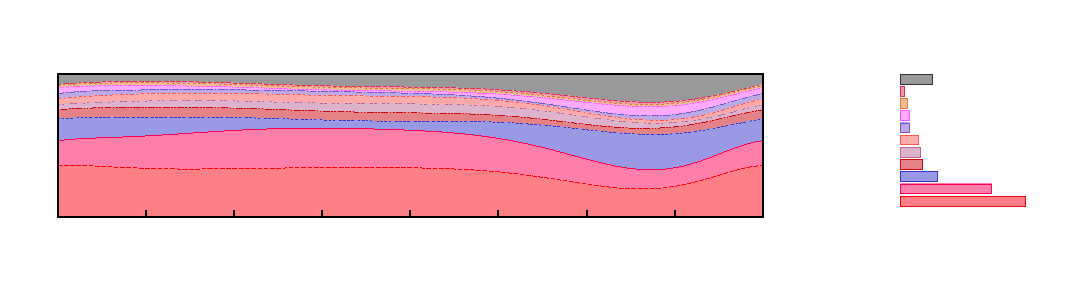
\includegraphics{img/zh}}%
    \gplfronttext
  \end{picture}%
\endgroup


\noindent% GNUPLOT: LaTeX picture with Postscript
\begingroup
  \makeatletter
  \providecommand\color[2][]{%
    \GenericError{(gnuplot) \space\space\space\@spaces}{%
      Package color not loaded in conjunction with
      terminal option `colourtext'%
    }{See the gnuplot documentation for explanation.%
    }{Either use 'blacktext' in gnuplot or load the package
      color.sty in LaTeX.}%
    \renewcommand\color[2][]{}%
  }%
  \providecommand\includegraphics[2][]{%
    \GenericError{(gnuplot) \space\space\space\@spaces}{%
      Package graphicx or graphics not loaded%
    }{See the gnuplot documentation for explanation.%
    }{The gnuplot epslatex terminal needs graphicx.sty or graphics.sty.}%
    \renewcommand\includegraphics[2][]{}%
  }%
  \providecommand\rotatebox[2]{#2}%
  \@ifundefined{ifGPcolor}{%
    \newif\ifGPcolor
    \GPcolorfalse
  }{}%
  \@ifundefined{ifGPblacktext}{%
    \newif\ifGPblacktext
    \GPblacktexttrue
  }{}%
  % define a \g@addto@macro without @ in the name:
  \let\gplgaddtomacro\g@addto@macro
  % define empty templates for all commands taking text:
  \gdef\gplbacktext{}%
  \gdef\gplfronttext{}%
  \makeatother
  \ifGPblacktext
    % no textcolor at all
    \def\colorrgb#1{}%
    \def\colorgray#1{}%
  \else
    % gray or color?
    \ifGPcolor
      \def\colorrgb#1{\color[rgb]{#1}}%
      \def\colorgray#1{\color[gray]{#1}}%
      \expandafter\def\csname LTw\endcsname{\color{white}}%
      \expandafter\def\csname LTb\endcsname{\color{black}}%
      \expandafter\def\csname LTa\endcsname{\color{black}}%
      \expandafter\def\csname LT0\endcsname{\color[rgb]{1,0,0}}%
      \expandafter\def\csname LT1\endcsname{\color[rgb]{0,1,0}}%
      \expandafter\def\csname LT2\endcsname{\color[rgb]{0,0,1}}%
      \expandafter\def\csname LT3\endcsname{\color[rgb]{1,0,1}}%
      \expandafter\def\csname LT4\endcsname{\color[rgb]{0,1,1}}%
      \expandafter\def\csname LT5\endcsname{\color[rgb]{1,1,0}}%
      \expandafter\def\csname LT6\endcsname{\color[rgb]{0,0,0}}%
      \expandafter\def\csname LT7\endcsname{\color[rgb]{1,0.3,0}}%
      \expandafter\def\csname LT8\endcsname{\color[rgb]{0.5,0.5,0.5}}%
    \else
      % gray
      \def\colorrgb#1{\color{black}}%
      \def\colorgray#1{\color[gray]{#1}}%
      \expandafter\def\csname LTw\endcsname{\color{white}}%
      \expandafter\def\csname LTb\endcsname{\color{black}}%
      \expandafter\def\csname LTa\endcsname{\color{black}}%
      \expandafter\def\csname LT0\endcsname{\color{black}}%
      \expandafter\def\csname LT1\endcsname{\color{black}}%
      \expandafter\def\csname LT2\endcsname{\color{black}}%
      \expandafter\def\csname LT3\endcsname{\color{black}}%
      \expandafter\def\csname LT4\endcsname{\color{black}}%
      \expandafter\def\csname LT5\endcsname{\color{black}}%
      \expandafter\def\csname LT6\endcsname{\color{black}}%
      \expandafter\def\csname LT7\endcsname{\color{black}}%
      \expandafter\def\csname LT8\endcsname{\color{black}}%
    \fi
  \fi
  \setlength{\unitlength}{0.0500bp}%
  \begin{picture}(10080.00,2520.00)%
    \gplgaddtomacro\gplbacktext{%
      \csname LTb\endcsname%
      \put(176,1281){\rotatebox{-270}{\makebox(0,0){\strut{}\scriptsize fraction of tweets}}}%
      \put(3779,154){\makebox(0,0){\strut{}\scriptsize time of day (UTC)}}%
      \put(3779,2189){\makebox(0,0){\strut{}Countries that Tweet in und}}%
    }%
    \gplgaddtomacro\gplfronttext{%
      \csname LTb\endcsname%
      \put(396,374){\makebox(0,0){\strut{}\scriptsize 0:00}}%
      \put(1242,374){\makebox(0,0){\strut{}\scriptsize 3:00}}%
      \put(2088,374){\makebox(0,0){\strut{}\scriptsize 6:00}}%
      \put(2934,374){\makebox(0,0){\strut{}\scriptsize 9:00}}%
      \put(3780,374){\makebox(0,0){\strut{}\scriptsize 12:00}}%
      \put(4625,374){\makebox(0,0){\strut{}\scriptsize 15:00}}%
      \put(5471,374){\makebox(0,0){\strut{}\scriptsize 18:00}}%
      \put(6317,374){\makebox(0,0){\strut{}\scriptsize 21:00}}%
      \put(7163,374){\makebox(0,0){\strut{}\scriptsize 24:00}}%
    }%
    \gplgaddtomacro\gplbacktext{%
      \csname LTb\endcsname%
      \put(9083,154){\makebox(0,0){\strut{}~~}}%
      \put(9083,2189){\makebox(0,0){\strut{} }}%
    }%
    \gplgaddtomacro\gplfronttext{%
      \csname LTb\endcsname%
      \put(8352,751){\makebox(0,0)[r]{\strut{}\scriptsize~USA}}%
      \put(8352,868){\makebox(0,0)[r]{\strut{}\scriptsize~Brazil}}%
      \put(8352,985){\makebox(0,0)[r]{\strut{}\scriptsize~UK}}%
      \put(8352,1102){\makebox(0,0)[r]{\strut{}\scriptsize~Spain}}%
      \put(8352,1219){\makebox(0,0)[r]{\strut{}\scriptsize~Saudi~Arabia}}%
      \put(8352,1337){\makebox(0,0)[r]{\strut{}\scriptsize~Philippines}}%
      \put(8352,1454){\makebox(0,0)[r]{\strut{}\scriptsize~India}}%
      \put(8352,1571){\makebox(0,0)[r]{\strut{}\scriptsize~TR}}%
      \put(8352,1688){\makebox(0,0)[r]{\strut{}\scriptsize~Argentina}}%
      \put(8352,1805){\makebox(0,0)[r]{\strut{}\scriptsize~Mexico}}%
      \put(8352,1922){\makebox(0,0)[r]{\strut{}\scriptsize~other}}%
    }%
    \gplbacktext
    \put(0,0){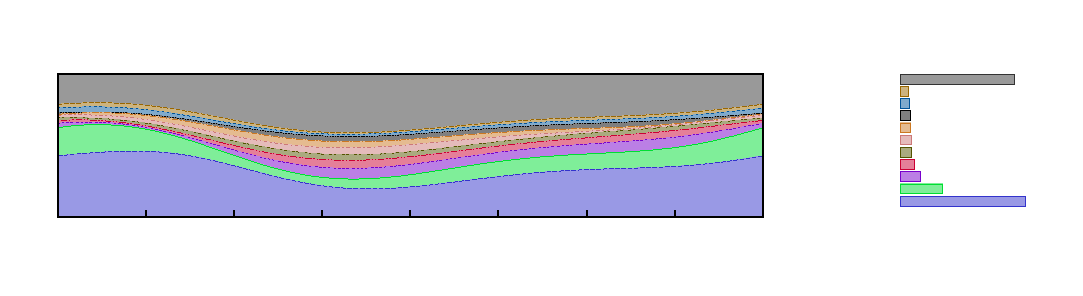
\includegraphics{img/und}}%
    \gplfronttext
  \end{picture}%
\endgroup



%%%%%%%%%%%%%%%%%%%%%%%%%%%%%%%%%%%%%%%%%%%%%%%%%%%%%%%%%%%%%%%%%%%%%%%%%%%%%%%%

\section{Reference notes}

%%%%%%%%%%%%%%%%%%%%%%%%%%%%%%%%%%%%%%%%

\subsection{Languages}

\citet{zaidan2014arabic} Arabic dialects.

\citet{refaee2014arabic} Arabic with twitter.

\citet{mohammad2016translation} translation alters sentiment.

%%%%%%%%%%%%%%%%%%%%%%%%%%%%%%%%%%%%%%%%

\subsection{Twitter applications}

\citet{cheng2010you} uses a probabilistic framework to generate city-level user home location using only tweet text.
Introduces a naive bayes model, but for some reason uses a sum instead of a product (bad math?).
Shows that this model does poorly,
and introduces a 'local words' weighting of the naive model to improve performance.
Introduces several smoothing mechanisms to help with the sparsity of tweet data.
They only consider tweets in the contiguous US.

\citet{kinsella2011m} predicts the location of individual tweets and a user's home location.
Provides a simple probabilistic model: 
For each location, estimate a distribution of terms associated with that location.
Does not incorporate time.
A straightforward generalization of \citet{cheng2010you} to tweet location instead of user location.

\citet{li2012towards} uses a probabilistic framework to generate city-level location using the content of the tweet and the network of tweet replies.
Does not use a gazetteer or the underlying social graph.
This seems like a straightforward extension of \citet{cheng2010you}.

\citet{han2013stacking} predicts the city of a twitter user using both text and metadeta using stacking.
I believe this is the first paper to consider the effect of semantic shift in geolocation.
They show that user declared location metadeta is more sensitive to temporal change than the message text.

\citet{mahmud2014home} identifies the home location of a user rather than the location of an individual tweet.
Incorporates temporal information in the tweets to identify when a user is travelling.
\fixme{Has good twitter geolocation references that I don't have elsewhere.}
Uses an ensemble classifier with a gazeteer as one of the key features.
Lots of manual constructions and NLP-based preprocessing.
Hierarchical model that first predicts a general geographic region (e.g. timezone or state), then predicts the city.

\citet{han2014text} has many new ideas.
Introduce a multilingual dataset and the first methods for geolocating non-English tweets.
They use a hierarchical model that first determines the language,
then selects a model appropriate for the language.
Make heavy use of twitter metadata (e.g. tweet time) to determine location.
Perform a test on time where they evaluate their model on data collected 1 year after the training data, and show a significant performance loss.
Studies the privacy implications of geolocation.

\citet{compton2014geotagging} propose a simple convex problem for geolocating twitter users to city level accuracy using the social network graph only.
Whereas previous methods rely on local heuristics, their convex program uses global properties of the social graph.
Has lots of empirical results showing accuracy of self reported locations, location homophily among friends, and typical travel habits of twitter users.

\citet{rahimi2015twitter} uses both twitter text and the network graph for geolocation, but does not include time.
\fixme{Has good twitter geolocation references that I don't have elsewhere.}
Good experiments with good datasets.
Uses kd-tree for faster search.
Spatial labels are discretized over an adaptive grid based on the number of users in the region.
The @-mention information is used to build an undirected graph between users.
They convert the graph into a ``collapsed graph'', and there's lots of subtleties here about how they handle the train/test split and edges that pass between the two sets.
Uses Model Adsorption over the graph to predict geolocations within the test set, 
with two key modification:
(i) removing celebrity nodes from the network graph (lets them scale to larger networks)
and (ii) incorporating textual information as ``dongle nodes''.

\citet{dredze2016geolocation} studies time's effect on geolocation of individual tweets to the city level.
Demonstrates cyclical temporal effects on geolocation accuracy and rapid drops in accuracy as test data moves beyond the training data's time period.
They show that this temporal drift can be countered with modest online model updates.
Introduces a particularly large new dataset.
Used vowpal wabbit to learn the model.

\citet{duong2016near} does regression to predict the gps coordinates without taking into account the geometry of the earth.
Uses matrix factorization of a bag-of-words type model.

%%%%%%%%%%%%%%%%%%%%%%%%%%%%%%%%%%%%%%%%

\subsection{Twitter analytics}

\citet{hecht2011tweets} measures the accuracy of the location field in twitter user profiles.

\citet{dredze2013carmen} introduces the Carmen system for twitter geolocation.
Then use it to improve influenza surveillance.
Carmen does not do prediction of location from text,
but instead only measures accuracy of the various location fields.

\citet{he2015hawkestopic} uses Hawkes process to model the social graph of Twitter,
but does not apply the idea to geolocation.

\citet{graham2014world} survey of geolocation methods for geographers.

%%%%%%%%%%%%%%%%%%%%%%%%%%%%%%%%%%%%%%%%

\subsection{Emojis}

\citet{park2013emoticon} studies emoticon usage in the first three years of the twitter platform.
They show, for example, that vertical emoticons are indicative of asian cultures and horizontal emoticons of european cultures.

\citet{lu2016learning} show that emoji usage varies around the world on smart phone SMS messages using a keyboard app.

\citet{ljubevsic2016global} shows that emoji usage can be used to predict tweet location.

%%%%%%%%%%%%%%%%%%%%%%%%%%%%%%%%%%%%%%%%

\subsection{Generic applications}

\citet{eisenstein2010latent} presents a multilevel generative model that resents jointly about latent topics and geographical regions.
Highly cited, and probably the right foundation for my graphical model.
Does not incorporate time or model the geometry of the regions.
Uses mean field variational inference.
\fixme{Think about this more.}

\citet{speriosu2010connecting} models language and geography outside the Twitter context for toponym resolution (disambiguating place names).
Uses a graphical model based on probabalistic topic models,
where regions of the earth are represented by different topics.
Inference is done with a collapsed Gibbs sampler.
Does not incorporate the Earth's spherical geometry or any distance relations between locations.

\citet{wu2017link} proposes a model for predicting the generation of new links in social networks. 
Uses a convex optimization problem with closed form solution.

\citet{yu2017temporally} uses matrix factorization to predict the formation of new edges in social networks.

%%%%%%%%%%%%%%%%%%%%%%%%%%%%%%%%%%%%%%%%

\subsection{Less important work}

\citet{leidner2011detecting} provides a tutorial on methods for parsing geographical references in natural language.

\citet{jurgens2015geolocation} surveys existing methods.
They show a large performance gap between real world performance and the idealized laboratory-performance reported in the compared methods' publications.
\fixme{Review their references}

%%%%%%%%%%%%%%%%%%%%%%%%%%%%%%%%%%%%%%%%

\subsection{Other applications of social network analysis}

\citet{ruiz2012correlating} uses tweets to predict financial markets.

\citet{wiley2014pharmaceutical} uses tweets to measure the effectiveness and user satisfaction of new drugs.

%%%%%%%%%%%%%%%%%%%%%%%%%%%%%%%%%%%%%%%%

\subsection{Deep learning}

\citet{kim2016character} proposes using character level CNNs, RNNs, and Highway Networks for language translation.
\citet{chung2016character} also proposes character level RNNs and highway nets for translation.
\citet{jozefowicz2016exploring} is a generic classification paper for character level text processing.  
Uses a combination of CNNs and RNNs, and a hierarchical softmax which might be useful for locations.

\citet{dhingra2016tweet2vec} creates a vector space model of tweets using a character level recurrent GRU network.
\citet{severyn2015unitn} use a word level CNN for sentiment classification on tweets.

\citet{conneau2017very} use resnet like connections to create very deep character cnns for text classification.
\citet{zhang2015character} use a smaller depth character CNN, which is what I've implemented so far.

\citet{weyand2016planet} do geolocation of photos using image CNNs.
They divide the globe into 26263 regions, and use a xentropy loss over those regions.
Regions are of different sizes so that they all contain approximately the same number of photos.

%%%%%%%%%%%%%%%%%%%%%%%%%%%%%%%%%%%%%%%%%%%%%%%%%%%%%%%%%%%%%%%%%%%%%%%%%%%%%%%%

\clearpage
\bibliography{paper}

%%%%%%%%%%%%%%%%%%%%%%%%%%%%%%%%%%%%%%%%%%%%%%%%%%%%%%%%%%%%%%%%%%%%%%%%%%%%%%%%

\end{document}
